\chapter{LQR-VMC平衡算法设计}\label{chap:controller}

本章在第三章建模结果的基础上，围绕双轮足机器人控制系统的实际需求，对整机控制策略进行重新组织与实现。结合前文对双轮足机器人运动特点的分析，本文采用一种分层轻量级混合控制方案：以 LQR 作为运动控制器，以 VMC 负责腿长方向支撑控制，并通过滚转补偿增强侧向稳定性。该结构兼顾了控制性能、参数可调性和实时实现难度，为本章 MuJoCo 仿真和第五章物理样机实验提供方法基础。

\section{总体架构}

双轮足机器人在实际运行中需要同时满足多类控制目标：其一，机器人应在前进方向上保持倒立摆平衡，并能够完成原地站立、速度跟踪和外部扰动恢复；其二，腿部机构应承担支撑、缓冲、抬升和摆动等局部任务，以保证整机高度调节和越障动作的可实现性；其三，机器人在转向、坡面运动和侧向扰动下还需要维持滚转稳定，避免出现单侧轮卸载或机体侧翻风险；其四，所有控制算法都需要满足样机嵌入式实时运行的要求，即在有限计算资源下完成状态估计、控制求解和执行器命令下发。

从控制效果看，WBC、MPC 等优化型方法能够较完整地处理多任务协调与约束，但这类方法通常依赖更精确的整机模型和更高的在线计算能力，
对本样机平台而言实现复杂度较高，也不符合轻量级控制策略的需求。
相比之下，LQR 适合处理平衡点附近的姿态稳定、速度调节和腿摆控制量分配问题，VMC 更适合在腿长方向构造支撑和缓冲行为。
因此，本文不采用“大而全”的统一优化框架，而是按照控制任务的物理属性将系统拆分为不同层级，在保证控制效果的同时降低在线求解负担。

综合上述考虑，本文构建的分层控制系统可概括为以下三层：
\begin{enumerate}
  \item 状态估计层：融合编码器和惯性测量单元信息，实时获得机体姿态、轮组位移、腿长、腿摆角及其变化率；
  \item 运动控制层：基于线性化状态空间模型设计 LQR 反馈律，生成轮系名义驱动力矩和腿摆控制量；
  \item 任务空间控制层：基于 VMC 构造腿长支撑力，并结合 LQR 给出的腿摆控制量完成任务空间到关节空间的力矩映射。
\end{enumerate}

\begin{figure}[H]
  \centering
  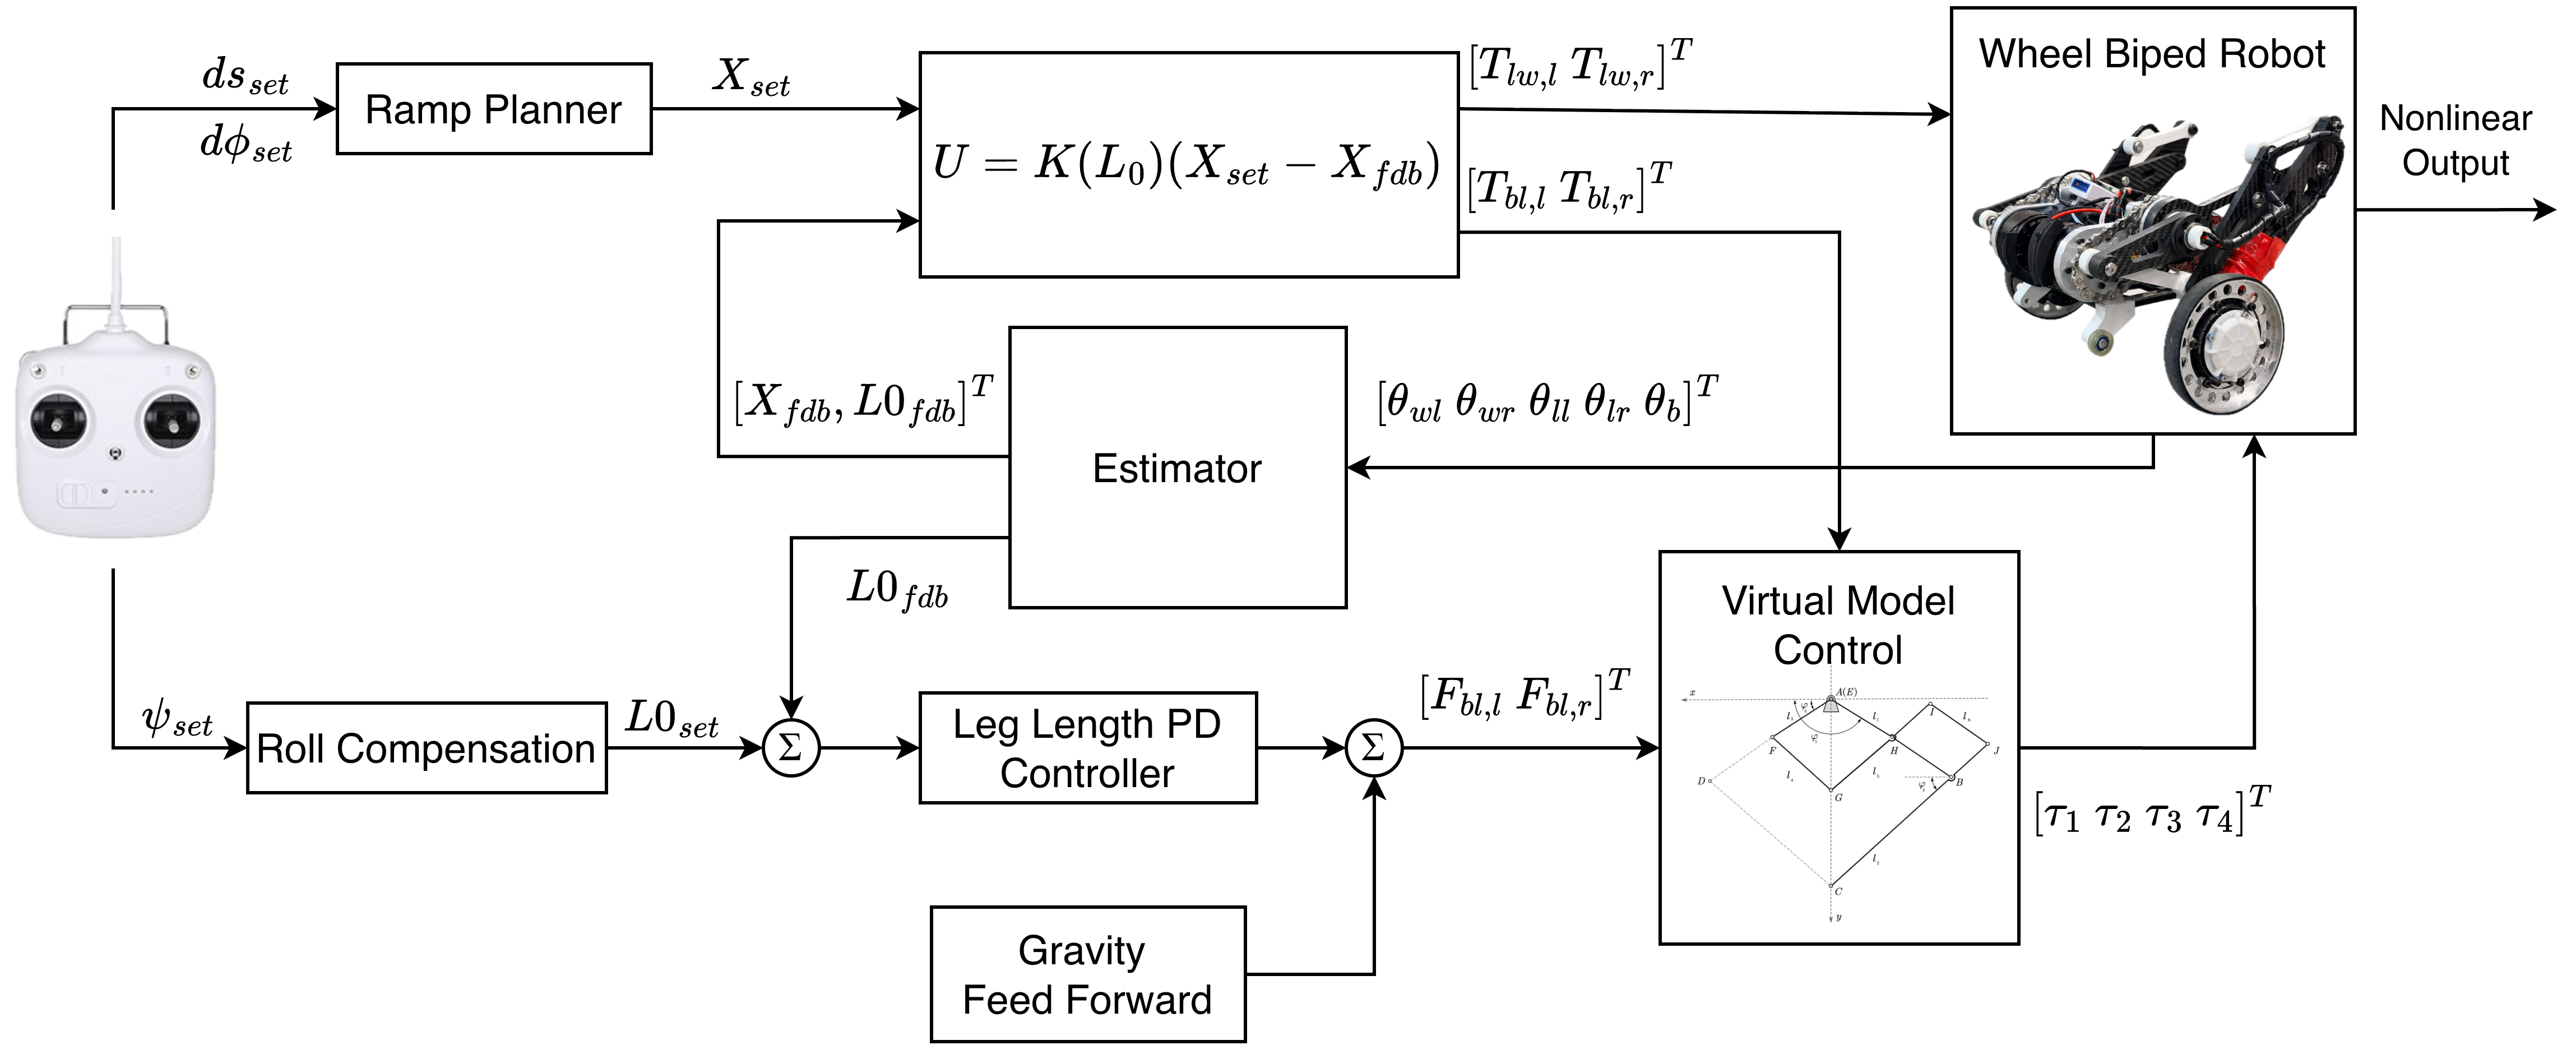
\includegraphics[width=1.0\textwidth]{figures/ch04/control_structure.png}
  \caption{整体控制框图}
  \label{fig:control-structure}
\end{figure}

上述架构的核心思想在于“全局平衡与局部支撑解耦”。其中，LQR 负责处理整机平衡、运动趋势和腿摆控制量，VMC 负责处理腿长方向的局部支撑行为，滚转补偿负责补足运动模型未展开的侧向稳定问题。这样既保持了控制结构清晰，又能体现本文“轻量级、可实时部署”的方法定位。

\section{LQR 控制器设计}

\subsection{控制目标与状态变量选取}

在分层控制框架中，运动控制器负责机器人在前进方向上的站立平衡、速度跟踪以及扰动恢复。考虑到机器人在直立工况附近可近似为多输入多输出线性系统，本文将第三章建立的五自由度动力学模型在线性化后用于 LQR 设计。为保持与原始模型的一致性，仍选取左右轮转角、左右腿摆角和机体俯仰角作为独立广义坐标，即
\begin{equation}
  \boldsymbol{q} =
  \begin{bmatrix}
    \theta_{wl} & \theta_{wr} & \theta_{ll} & \theta_{lr} & \theta_b
  \end{bmatrix}^{\mathsf{T}}
  \label{eq:full-generalized-coordinate}
\end{equation}
输入向量定义为
\begin{equation}
  \boldsymbol{u} =
  \begin{bmatrix}
    T_{lw,l} & T_{lw,r} & T_{bl,l} & T_{bl,r}
  \end{bmatrix}^{\mathsf{T}}
  \label{eq:full-input-vector}
\end{equation}

为了使状态量更贴近机器人实际运动状态，本文将前进位移 $s$、偏航角 $\phi$、左右腿摆角和机体俯仰角作为控制器设计中的物理状态，并构造完整状态向量
\begin{equation}
  \boldsymbol{x}
  =
  \begin{bmatrix}
    s & \dot{s} & \phi & \dot{\phi} & \theta_{ll} & \dot{\theta}_{ll} &
    \theta_{lr} & \dot{\theta}_{lr} & \theta_b & \dot{\theta}_b
  \end{bmatrix}^{\mathsf{T}}.
  \label{eq:full-state-vector}
\end{equation}
其中，$s$ 与 $\phi$ 由第三章给出的轮系运动学关系计算得到。相较于直接使用广义坐标，\eqref{eq:full-state-vector} 中的状态量具有更清晰的物理意义，更便于从“平衡、转向、腿摆、俯仰”四类目标出发进行权重设计和实验分析。

\subsection{线性状态空间模型构建}

选取机器人静态直立工况作为平衡工作点，对第三章推导得到的非线性动力学方程进行小角度线性化，可得广义动力学形式
\begin{equation}
  \boldsymbol{M}\ddot{\boldsymbol{q}} + \boldsymbol{K}\boldsymbol{q} = \boldsymbol{E}\boldsymbol{u},
  \label{eq:linearized-generalized-dynamics}
\end{equation}
其中，$\boldsymbol{M}$ 为平衡点处的等效惯性矩阵，$\boldsymbol{K}$ 为线性化后的重力与耦合项矩阵，$\boldsymbol{E}$ 为输入分配矩阵。由 $\boldsymbol{M}$ 的非奇异性，可将上式改写为显式加速度形式
\begin{equation}
  \ddot{\boldsymbol{q}}
  =
  \boldsymbol{A}_{\mathrm{dyn}} \boldsymbol{q}
  +
  \boldsymbol{B}_{\mathrm{dyn}} \boldsymbol{u}
  \qquad
  \boldsymbol{A}_{\mathrm{dyn}} = -\boldsymbol{M}^{-1}\boldsymbol{K}
  \qquad
  \boldsymbol{B}_{\mathrm{dyn}} = \boldsymbol{M}^{-1}\boldsymbol{E}
  \label{eq:qdd-dyn}
\end{equation}

第三章已经给出轮系与腿部运动学映射关系，因此前进位移和偏航角满足
\begin{equation}
  s = \frac{R_w}{2}\left(\theta_{wl} + \theta_{wr}\right)
  \label{eq:s-kinematic-map}
\end{equation}
\begin{equation}
  \phi
  =
  \frac{R_w}{2R_l}\left(-\theta_{wl} + \theta_{wr}\right)
  -
  \frac{l_l}{2R_l}\sin \theta_{ll}
  +
  \frac{l_r}{2R_l}\sin \theta_{lr}
  \label{eq:phi-kinematic-map}
\end{equation}
在平衡点附近将\eqref{eq:s-kinematic-map} 和\eqref{eq:phi-kinematic-map} 线性化，并将广义坐标表达式转换为\eqref{eq:full-state-vector} 所示的物理状态后，主控制器使用的标准状态空间方程可写为
\begin{equation}
  \dot{\boldsymbol{x}} = \boldsymbol{A}\boldsymbol{x} + \boldsymbol{B}\boldsymbol{u}
  \label{eq:linear-state-space}
\end{equation}

\eqref{eq:linear-state-space} 给出了用于运动控制器设计的线性模型。与原始非线性模型相比，该表达式在保留轮系、腿部和俯仰耦合关系的同时，显著降低了在线求解难度。

\subsection{LQR 反馈律设计}

对于\eqref{eq:linear-state-space} 描述的十维四输入线性时不变系统，本文采用线性二次型调节器（LQR）作为运动控制器\cite{klemm2020lqr}。
选择 LQR 的原因在于：一方面，机器人在站立与匀速行进工况下的大部分控制任务均围绕直立平衡点展开，线性模型能够较好描述该工作区间内的主要动力学特性；另一方面，LQR 仅需离线求解 Riccati 方程，在线阶段只进行矩阵乘法运算，计算量小，便于嵌入式实时实现。

定义无穷时域二次性能指标为
\begin{equation}
  J =
  \int_{0}^{\infty}
  \left(
    \delta \boldsymbol{x}^{\mathsf{T}}\boldsymbol{Q}\,\delta \boldsymbol{x}
    +
    \delta \boldsymbol{u}^{\mathsf{T}}\boldsymbol{R}\,\delta \boldsymbol{u}
  \right)\dd t,
  \label{eq:lqr-cost}
\end{equation}
其中，$\boldsymbol{Q} \succeq 0$ 为状态加权矩阵，$\boldsymbol{R} \succ 0$ 为控制加权矩阵。$\boldsymbol{Q}$ 用于度量前进位移、偏航角、腿摆角和机体俯仰角等状态的偏差程度；$\boldsymbol{R}$ 用于约束轮电机与腿部驱动器的输出幅值，避免过大的控制输入导致执行器饱和和结构冲击。在实际设计中，可适当增大 $\theta_b$、$\dot{\theta}_b$ 和 $\dot{s}$ 的权重，以提高姿态稳定与速度恢复能力。

对于增量系统
\begin{equation}
  \delta \dot{\boldsymbol{x}}
  =
  \boldsymbol{A}\delta \boldsymbol{x}
  +
  \boldsymbol{B}\delta \boldsymbol{u},
  \label{eq:lqr-system}
\end{equation}
若存在正定矩阵 $\boldsymbol{P}$ 满足连续时间代数 Riccati 方程
\begin{equation}
  \boldsymbol{A}^{\mathsf{T}}\boldsymbol{P}
  +
  \boldsymbol{P}\boldsymbol{A}
  -
  \boldsymbol{P}\boldsymbol{B}\boldsymbol{R}^{-1}\boldsymbol{B}^{\mathsf{T}}\boldsymbol{P}
  +
  \boldsymbol{Q}
  =
  \boldsymbol{0},
  \label{eq:riccati}
\end{equation}
则最优状态反馈律为
\begin{equation}
  \delta \boldsymbol{u}
  =
  -\boldsymbol{K}\delta \boldsymbol{x},
  \qquad
  \boldsymbol{K} =
  \boldsymbol{R}^{-1}\boldsymbol{B}^{\mathsf{T}}\boldsymbol{P}.
  \label{eq:lqr-law}
\end{equation}
因此主控制器输出可写为
\begin{equation}
  \boldsymbol{u}
  =
  \begin{bmatrix}
    T_{lw,l} & T_{lw,r} & T_{bl,l} & T_{bl,r}
  \end{bmatrix}^{\mathsf{T}}
  =
  -
  \boldsymbol{K}
  \left(
    \boldsymbol{x} - \boldsymbol{x}_d
  \right),
  \label{eq:lqr-output}
\end{equation}
其中，$\boldsymbol{x}_d$ 为期望状态向量。静态站立任务中通常取 $\boldsymbol{x}_d = \boldsymbol{0}$；速度跟踪或转向任务中，则可通过设置 $\dot{s}_d$、$\phi_d$ 等参考量生成相应的平衡工作点。

\section{VMC 控制器设计}

\subsection{腿长控制律}

LQR 主控制器能够有效处理前进方向上的全局平衡，但它并不直接负责腿长调节、缓冲支撑和越障时的局部运动组织。
考虑到闭环五连杆机构在关节空间中耦合较强，而虚拟腿长度和虚拟腿摆角具有更明确的物理含义，本文在腿部控制中仍采用任务空间描述：腿长方向由 VMC 构造轴向支撑力，腿摆方向直接沿用 LQR 输出的控制量。

对于左、右腿，分别定义任务空间状态为
\begin{equation}
  \boldsymbol{x}_{v,i} =
  \begin{bmatrix}
    l_i & \theta_{l,i}
  \end{bmatrix}^{\mathsf{T}},
  \qquad i \in \{l,r\},
  \label{eq:leg-task-state}
\end{equation}
其中，$l_i$ 表示第 $i$ 条腿的虚拟腿长，$\theta_{l,i}$ 表示其虚拟腿摆角。针对腿长方向，构造虚拟弹簧阻尼器，并引入重力前馈补偿，其轴向虚拟力为
\begin{equation}
  F_{l,i}^{\ast}
  =
  K_l (l_{d,i} - l_i)
  +
  D_l (\dot{l}_{d,i} - \dot{l}_i)
  +
  \frac{1}{2} mg \cos\theta_{l,i},
  \qquad i \in \{l,r\}.
  \label{eq:leg-force-law}
\end{equation}
其中，$m$ 为机器人的部分或整体等效质量，$\frac{1}{2} m g \cos\theta_{l,i}$ 为在此摆角下单腿分担的重力前馈项。\eqref{eq:leg-force-law} 使腿部在支撑阶段表现为具有等效刚度和阻尼的虚拟支撑单元，从而实现机体高度维持、落地缓冲和腿长振荡抑制。与直接进行关节位置控制相比，这种写法更符合机器人与地面发生力学作用时的控制需求，也更便于在不同工况下通过少量参数完成行为切换。

在腿摆方向，本文不再额外构造 PD 修正项，而是直接采用 LQR 主控制器输出的对应腿部控制量。记任务空间中的腿摆虚拟转矩为 $T_{\theta,i}^{\ast}$，则有
\begin{equation}
  T_{\theta,i}^{\ast} = T_{bl,i}^{\ast},
  \qquad i \in \{l,r\}.
  \label{eq:leg-swing-lqr-input}
\end{equation}
其中，$T_{bl,i}^{\ast}$ 来自\eqref{eq:lqr-output}。这样处理可以避免在腿摆方向重复引入局部闭环，使腿摆控制量与线性化平衡模型中的输入保持一致。

因此，左右腿的任务空间控制量可写为
\begin{equation}
  \boldsymbol{F}_{v,i}^{\ast}
  =
  \begin{bmatrix}
    F_{l,i}^{\ast} \\
    T_{\theta,i}^{\ast}
  \end{bmatrix},
  \qquad i \in \{l,r\}.
  \label{eq:task-space-input}
\end{equation}

\subsection{任务空间到关节空间的力矩映射}

由第三章给出的虚拟腿雅可比矩阵 $\boldsymbol{J}_{v,i}$ 和虚功原理，任务空间控制量到实际关节空间的映射可写为
\begin{equation}
  \boldsymbol{\tau}_{i}^{\ast}
  =
  \boldsymbol{J}_{v,i}^{\mathsf{T}}\boldsymbol{F}_{v,i}^{\ast},
  \qquad i \in \{l,r\}.
  \label{eq:leg-joint-torque}
\end{equation}
其中，$\boldsymbol{\tau}_{i}^{\ast}$ 为第 $i$ 条腿对应主动关节的驱动力矩向量。\eqref{eq:leg-joint-torque} 将“任务空间中的腿长支撑力与 LQR 腿摆控制量”转换为“关节空间中的可执行力矩命令”，使闭环五连杆机构仍可在虚拟腿描述下进行直观控制。因此，本文并不在第四章重复推导闭环机构运动学细节，而是直接调用第三章建立的映射关系，以减少章节间重复。

\section{机体滚转角补偿}

第三章建立的主动力学模型主要刻画前进方向、腿摆和机体俯仰之间的耦合运动。根据第三章基本假设，整机主动力学分析中暂不展开滚转角、左右支撑力差异和侧向惯性力矩的影响。对于实际样机而言，这一模型已经能够覆盖站立和平地直行时的主要动力学特征，但在上下坡、单边桥、横向扰动和转向等工况下，机器人仍会出现明显的侧向滚转。特别是在转向速度较高时，向心力会改变左右侧的实际支撑状态。如果仍按水平地面条件分配推力并调节腿长，机体容易向外侧倾斜，左右腿支撑也会逐渐失衡，进而影响转向过程中的姿态稳定性。

基于上述考虑，本文在原有控制结构之外增加滚转角补偿环节，并采用一种基于几何关系的腿长差修正方法。其基本思路是：根据测得的滚转角以及当前左右腿的几何状态，计算出应施加的期望腿长差，再将这一修正量叠加到腿长通道参考值中，以抑制机体侧倾趋势。该方法不需要改动运动控制器和 VMC 的主体结构，实现上也较为直接，适合在嵌入式平台上实时运行。

在单边桥或侧向不平整地面工况下，机体滚转角可以理解为机器人相对于局部支撑平面的姿态偏差。设左右腿当前腿长分别为 $l_l$ 和 $l_r$，半轮距为 $b$，滚转角为 $\gamma$。由几何关系定义等效坡角 $\delta_{\mathrm{roll}}$，其正切形式为
\begin{equation}
  \tan \delta_{\mathrm{roll}}
  =
  \frac{
    (l_r-l_l)\cos\gamma + 2b\sin\gamma
  }{
    (l_l-l_r)\sin\gamma + 2b\cos\gamma
  }.
  \label{eq:roll-delta}
\end{equation}

进一步地，由右腿一侧的几何关系，机体中心相对于局部支撑平面的等效高度为
\begin{equation}
  h
  =
  l_r\cos\gamma + b\sin\gamma.
  \label{eq:roll-body-height}
\end{equation}
若希望机体在该等效坡面上保持水平，则左右腿的期望腿长可写为
\begin{equation}
  l_{d,l}^{\mathrm{roll}} = h,
  \qquad
  l_{d,r}^{\mathrm{roll}} = h - 2b\tan \delta_{\mathrm{roll}}.
  \label{eq:roll-leg-target}
\end{equation}
因此，由滚转角引起的期望腿长差为
\begin{equation}
  \Delta l_{\mathrm{roll}}
  =
  l_{d,l}^{\mathrm{roll}} - l_{d,r}^{\mathrm{roll}}
  =
  2b\tan \delta_{\mathrm{roll}}.
  \label{eq:roll-leg-diff}
\end{equation}

\eqref{eq:roll-leg-diff} 给出了该补偿方法的核心结果，即先由当前滚转角和左右腿几何关系求出等效坡角，再将其转化为左右腿的期望腿长差。考虑到腿长通道中已经存在基准腿长控制，为避免直接替换参考量引起指令突变，本文将腿长差的一半以相反符号叠加到左右腿基准腿长上，即
\begin{equation}
  l_{d,l} = l_d + \frac{1}{2}\Delta l_{\mathrm{roll}},
  \qquad
  l_{d,r} = l_d - \frac{1}{2}\Delta l_{\mathrm{roll}},
  \label{eq:roll-leg-superimpose}
\end{equation}
其中，$l_d$ 为对称支撑工况下的公共基准腿长。随后将 $l_{d,l}$ 和 $l_{d,r}$ 代入\eqref{eq:leg-force-law} 对应的左右腿腿长控制器，即可得到滚转补偿后的腿长控制量。

与前述 LQR 和 VMC 控制结构相比，这里的补偿不直接通过支撑力差动构造恢复力矩，而是通过调整左右腿的期望长度来改变局部支撑几何关系。这样处理有两个直接好处：一是物理意义清晰，便于解释单边桥和侧向地形下的姿态修正过程；二是计算量较小，只依赖滚转角、左右腿长和半轮距等基础状态量，便于在嵌入式系统中实现。对于转向工况中由推力变化带来的附加侧倾，\eqref{eq:roll-leg-superimpose} 同样可以作为腿长通道的在线修正项，与上层速度控制配合使用，以减小机体外倾趋势。

\section{状态估计器设计}

为支撑上述分层控制策略的在线运行，样机控制系统配置了轮组编码器、腿部关节编码器以及惯性测量单元等基础传感器。轮组编码器用于获取左右轮转角及其变化率；腿部关节编码器结合第三章建立的机构运动学关系，可实时解算左右腿的虚拟腿长 $l_i$、虚拟腿摆角 $\theta_{l,i}$ 及其导数；惯性测量单元用于获取机体俯仰角、滚转角、角速度以及机体加速度。由于轮腿机器人在越过地形突起或发生轻微打滑时，单纯由轮速积分得到的速度容易出现突变，本文在轮速运动学解算的基础上引入惯性加速度观测，并采用卡尔曼滤波（Kalman filter, KF）进行前进速度估计\cite{kalman1960new}。

在状态估计层中，本文需要为 LQR 主控制器提供前进位移 $s$、前进速度 $\dot{s}$、机体俯仰角 $\theta_b$、腿摆角及其变化率等状态，同时为 VMC 腿长控制提供左右腿长及其变化率。机体姿态主要由惯性测量单元获得；腿部任务空间状态由关节编码器和等效五连杆运动学关系解算；前进速度则由轮速解算值与机体惯性加速度融合得到。这样既避免了依赖外部定位系统，也能减小复杂地面接触造成的轮速测量突变。

考虑单侧驱动轮的运动关系。设轮毂电机编码器测得的转子相对定子的角速度为 $\omega_{\mathrm{enc}}$，腿部机构带动轮轴支架相对机体的角速度为 $\dot{\theta}_l$，机体相对惯性系的俯仰角速度为 $\dot{\theta}_b$。在轮端不打滑且近似纯滚动的条件下，驱动轮相对地面的角速度可近似写为
\begin{equation}
  \omega_w
  =
  \omega_{\mathrm{enc}}
  +
  \dot{\theta}_l
  +
  \dot{\theta}_b .
  \label{eq:wheel-ground-angular-velocity}
\end{equation}
由轮半径 $R_w$ 可得到轮轴接地点对应的平动速度
\begin{equation}
  \dot{x}_w = R_w \omega_w .
  \label{eq:wheel-velocity-est}
\end{equation}

对于本文采用的虚拟腿描述，机体质心前向位置与轮轴位置、虚拟腿长度和腿摆角之间存在几何关系。以单侧等效模型说明，若记虚拟腿长度为 $l$，腿摆角为 $\theta_l$，则机体前向速度可写为
\begin{equation}
  \dot{x}_b
  =
  \dot{x}_w
  +
  l \dot{\theta}_l \cos\theta_l
  +
  \dot{l}\sin\theta_l .
  \label{eq:body-velocity-kinematic}
\end{equation}
将\eqref{eq:wheel-velocity-est} 代入上式，即可得到由编码器和姿态角速度解算出的机体前进速度观测量。实际实现中，左右两侧轮组分别计算得到 $\dot{x}_{b,l}$ 和 $\dot{x}_{b,r}$，直线运动时取二者平均作为前进速度观测值
\begin{equation}
  \dot{s}_{\mathrm{enc}}
  =
  \frac{1}{2}
  \left(
    \dot{x}_{b,l}
    +
    \dot{x}_{b,r}
  \right).
  \label{eq:encoder-forward-velocity}
\end{equation}
同时，左右轮速度差可用于估计偏航角速度，并结合第三章轮系运动学关系得到偏航角 $\phi$ 及其变化率。

轮速运动学解算具有计算量小、响应快的优点，但其可靠性依赖纯滚动假设。当机器人经过地形突起、轮端短时离地或发生打滑时，轮速会出现瞬时突变，直接作为控制反馈可能导致轮端力矩反向冲击。为抑制该问题，本文将惯性测量单元得到的前向加速度作为第二类观测量，并构造二状态离散 KF 对前进速度进行递推估计。

定义观测器状态为
\begin{equation}
  \boldsymbol{x}_{o}
  =
  \begin{bmatrix}
    v & a
  \end{bmatrix}^{\mathsf{T}},
  \label{eq:observer-state}
\end{equation}
其中，$v$ 为机体前进速度，$a$ 为机体前向加速度。KF 的预测模型采用匀加速度离散模型，可写为
\begin{equation}
  \boldsymbol{x}_{o,k+1}
  =
  \boldsymbol{F}_k \boldsymbol{x}_{o,k}
  +
  \boldsymbol{\Gamma}_k w_k,
  \qquad
  w_k \sim \mathcal{N}(0,Q_k),
  \label{eq:observer-process}
\end{equation}
其中
\begin{equation}
  \boldsymbol{F}_k
  =
  \begin{bmatrix}
    1 & \Delta t \\
    0 & 1
  \end{bmatrix},
  \qquad
  \boldsymbol{\Gamma}_k
  =
  \begin{bmatrix}
    \frac{1}{2}\Delta t^2 \\
    \Delta t
  \end{bmatrix}.
  \label{eq:observer-matrix}
\end{equation}

KF 的观测向量由轮速运动学解算得到的速度 $\dot{s}_{\mathrm{enc}}$ 和惯性测量单元得到的前向加速度 $a_{\mathrm{imu}}$ 组成，即
\begin{equation}
  \boldsymbol{z}_k
  =
  \begin{bmatrix}
    \dot{s}_{\mathrm{enc}} \\
    a_{\mathrm{imu}}
  \end{bmatrix}
  =
  \boldsymbol{H}_k \boldsymbol{x}_{o,k}
  +
  \boldsymbol{v}_k,
  \qquad
  \boldsymbol{H}_k
  =
  \begin{bmatrix}
    1 & 0 \\
    0 & 1
  \end{bmatrix},
  \label{eq:observer-measurement}
\end{equation}
其中，$\boldsymbol{v}_k \sim \mathcal{N}(\boldsymbol{0},\boldsymbol{R}_k)$ 为测量噪声，测量噪声协方差可取为
\begin{equation}
  \boldsymbol{R}_k
  =
  \begin{bmatrix}
    \sigma_v^2 & 0 \\
    0 & \sigma_a^2
  \end{bmatrix}.
  \label{eq:observer-noise}
\end{equation}
这里，$\sigma_v^2$ 反映轮速解算结果的可信度，$\sigma_a^2$ 反映惯性加速度测量的噪声水平。KF 根据过程噪声协方差 $Q_k$ 和测量噪声协方差 $\boldsymbol{R}_k$ 在预测值与观测值之间分配权重。当地面接触较平稳时，可适当提高轮速观测的权重；当机器人经过凸起或存在打滑风险时，可增大 $\sigma_v^2$，使估计结果更多依赖惯性加速度预测，从而降低速度反馈中的瞬时尖峰。

经过上述估计后，控制器使用的前进速度取观测器输出的 $\hat{v}$，前进位移 $s$ 由 $\hat{v}$ 积分并结合轮系位移进行低频修正。机体俯仰角 $\theta_b$、滚转角 $\gamma$ 及其角速度由惯性测量单元提供，左右虚拟腿长 $l_i$、腿摆角 $\theta_{l,i}$ 及其导数由腿部关节编码器和运动学关系实时解算。最终，状态估计层向上层控制器输出
\begin{equation}
  \hat{\boldsymbol{x}}
  =
  \begin{bmatrix}
    \hat{s} & \hat{\dot{s}} & \hat{\phi} & \hat{\dot{\phi}} &
    \hat{\theta}_{l,l} & \hat{\dot{\theta}}_{l,l} &
    \hat{\theta}_{l,r} & \hat{\dot{\theta}}_{l,r} &
    \hat{\theta}_b & \hat{\dot{\theta}}_b
  \end{bmatrix}^{\mathsf{T}}.
  \label{eq:estimated-controller-state}
\end{equation}
该 KF 估计方式将编码器的快速响应与惯性测量的抗突变能力结合起来，能够为 LQR-VMC 控制器提供更平滑的速度反馈，并降低复杂地面接触对平衡控制的影响。

\section{MuJoCo仿真验证}

为在物理样机制作和进行实验前检查控制器的基本闭环行为并对机构合理性做出验证，
本文在 MuJoCo \cite{todorov2012mujoco}中建立双轮足机器人仿真模型，并将第三章和本章的控制变量与仿真模型中的关节、轮组和机体姿态相对应。
仿真验证的目的不是单独追求模型与样机的完全一致，而是检查设计的 LQR-VMC 分层控制器能否在典型工况下实现稳定闭环，并为后续样机调试提供参数初值和安全边界。

\subsection{仿真模型与控制器实现}

MuJoCo 仿真模型主要包括机体刚体、左右腿部连杆、足端轮组、转动关节、电机执行器以及地面接触参数。
机体质量、轮半径、轮距、腿部连杆尺寸和执行器力矩上限根据第二章样机设计参数设置；
腿部运动学关系则与第三章建立的等效五连杆模型保持一致。
由于本文控制器采用虚拟腿任务空间描述，仿真中不直接将腿部关节作为控制目标，
而是由关节角实时解算左右虚拟腿长 $l_i$、腿摆角 $\theta_{l,i}$ 及其变化率，再将 VMC 腿长输出和 LQR 腿摆输出组成任务空间控制量，并通过雅可比转置映射为关节力矩。

仿真控制器按固定周期1kHz运行。每个控制周期内，程序首先从 MuJoCo 读取机体姿态、轮角、轮速、腿部关节角和关节角速度；
随后完成前进位移、前进速度、虚拟腿长和腿摆角等状态估计；接着执行 LQR 反馈、VMC 腿长支撑计算以及任务空间力矩映射；
最后将轮端力矩和腿部关节力矩下发至 MuJoCo 执行器。该流程与前文控制系统在线工作流程一致，从而能够检验控制律在多刚体接触环境中的实际闭环效果。

\begin{figure}[H]
  \centering
  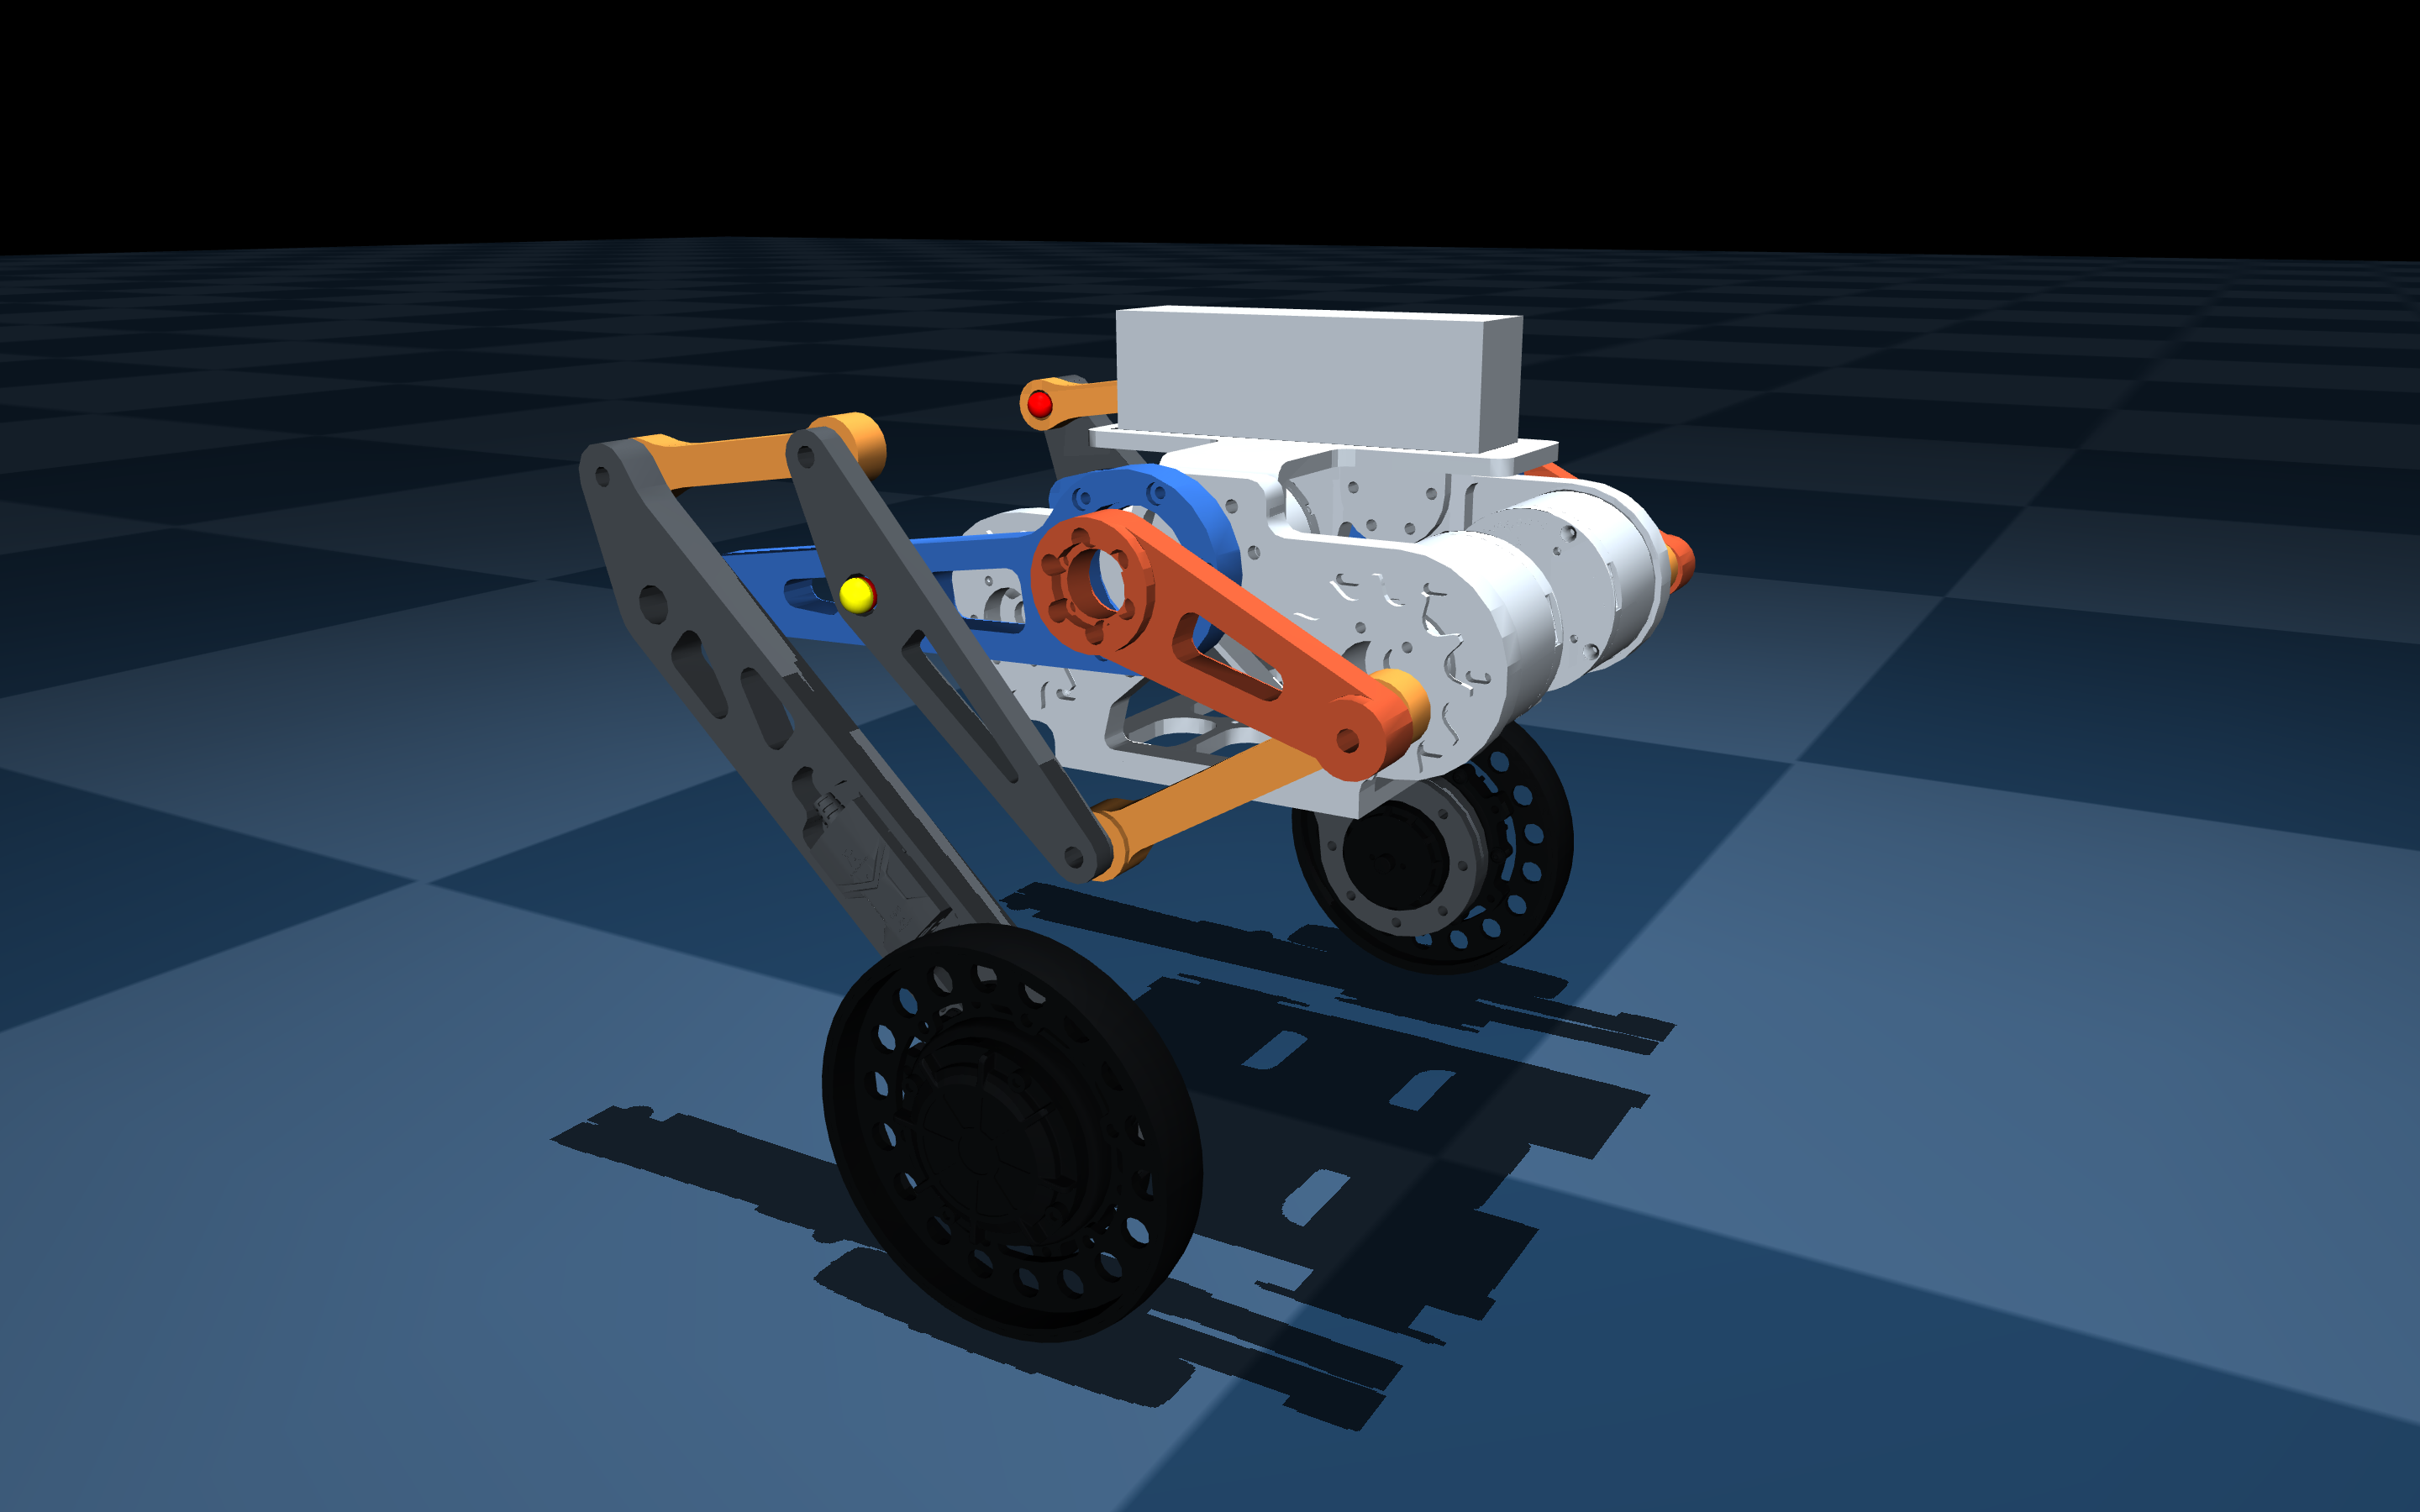
\includegraphics[width=0.95\textwidth]{figures/ch04/mujoco_model.png}
  \caption{MuJoCo 双轮足机器人仿真模型}
  \label{fig:mujoco-model}
\end{figure}

为评价不同控制环节的作用，本文主要记录机体俯仰角 $\theta_b$、前进速度 $\dot{s}$、期望腿长 $l_d$、实际腿长 $l_i$、腿长误差 $l_d-l_i$、轮端力矩 $T_{lw,i}$、腿部关节力矩 $\tau_i$ 。
上述指标分别对应平衡稳定性、速度跟踪能力、腿长调节能力和腿部支撑效果。

\subsection{原地平衡}

原地平衡仿真用于验证 LQR 主控制器与 VMC 腿长控制器能否在直立工作点附近形成稳定闭环。仿真初始时刻给机器人施加一定机体俯仰角偏差，期望前进速度取 $\dot{s}_d=0$，期望偏航角和腿摆角取零，左右腿期望腿长均取基准腿长 $l_d$。控制器启动后，LQR 根据俯仰角、俯仰角速度和轮系状态生成轮端力矩，VMC 则维持左右腿长在期望值附近。

\begin{figure}[H]
  \centering
  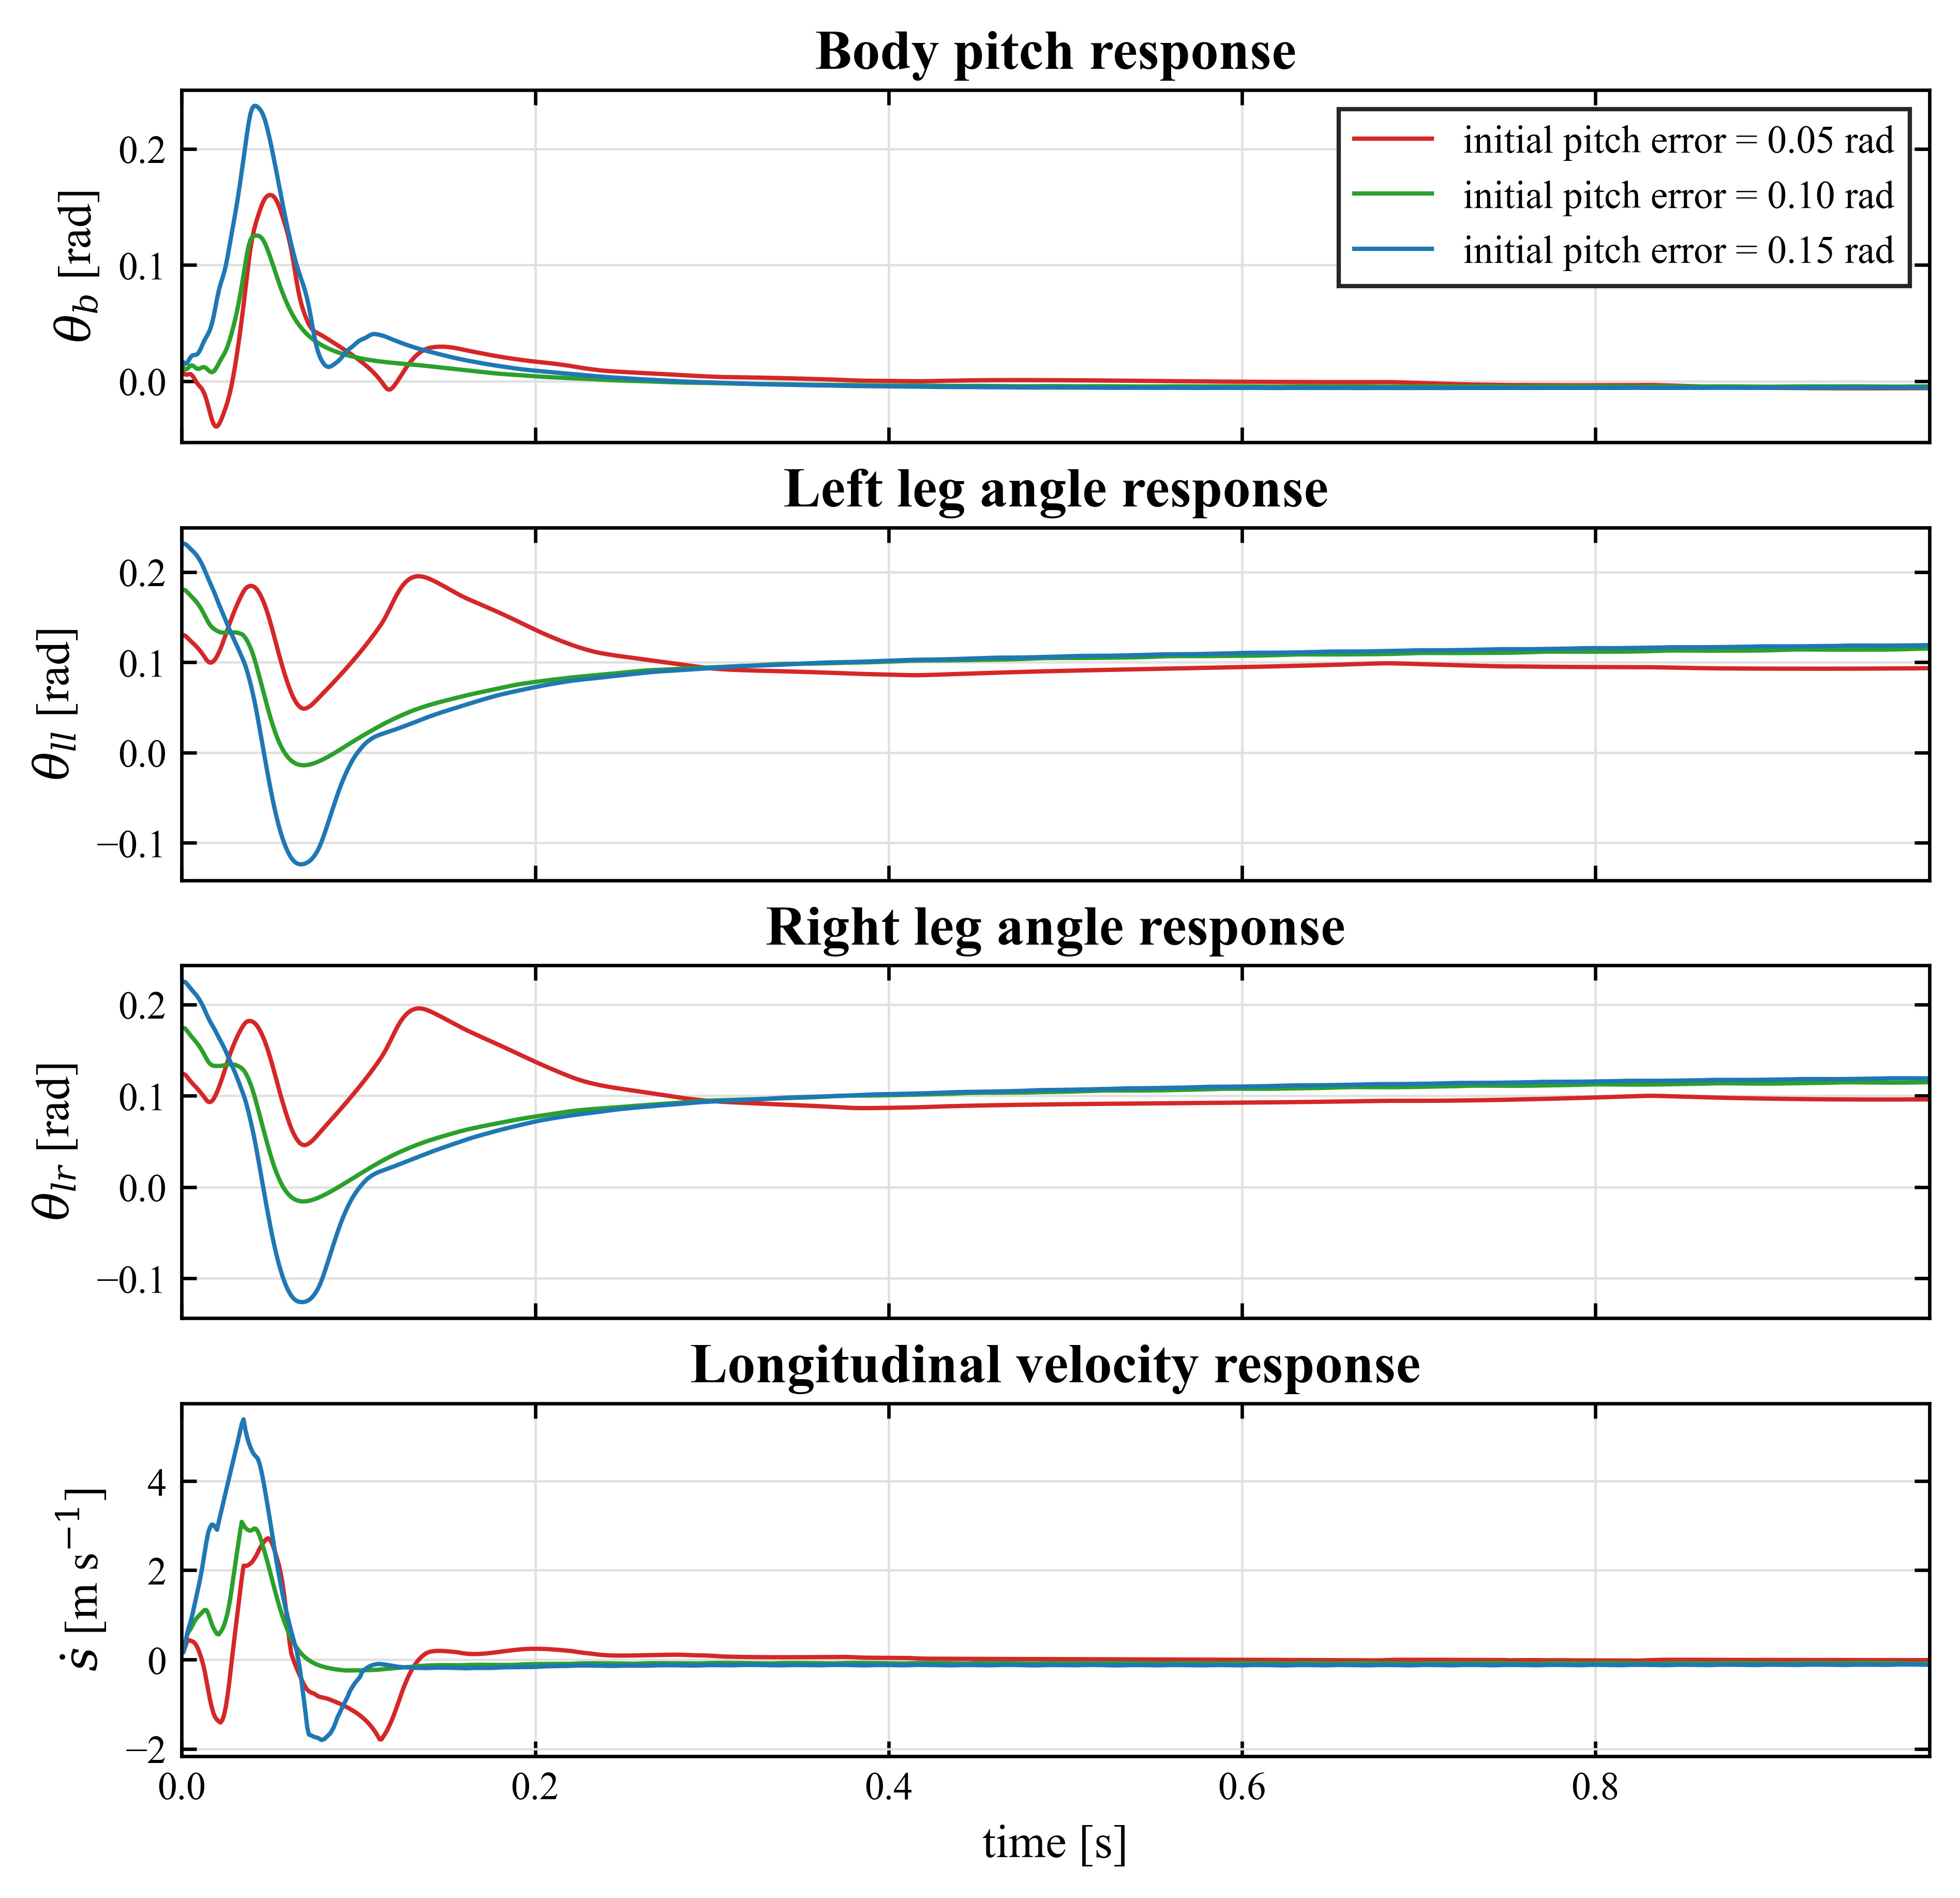
\includegraphics[width=1.0\textwidth]{figures/ch04/balance_response.png}
  \caption{原地平衡工况下的闭环响应。从上至下分别为机体俯仰角、左右腿角、水平速度}
  \label{fig:balance-response}
\end{figure}

仿真结果显示机体俯仰角在0.4s后收敛、左右腿角在0.3s后收敛，水平速度在0.2后收敛。整个控制过程没有明显震荡超调。
说明 LQR 与 VMC 在站立工况下能够协同工作，符合轮式倒立摆通过轮端运动调节机体姿态的物理规律。

\subsection{速度跟踪}

速度跟踪仿真用于检验 LQR 控制器对前进速度和机体姿态的协调能力。仿真中先令机器人保持原地平衡，随后给定水平阶跃速度参考，
由 $0$ 切换至正向速度 $\dot{s}_d$。该工况下，机器人需要通过短时俯仰角偏转产生加速度，并在速度接近期望值后重新回到直立平衡附近。

\begin{figure}[H]
  \centering
  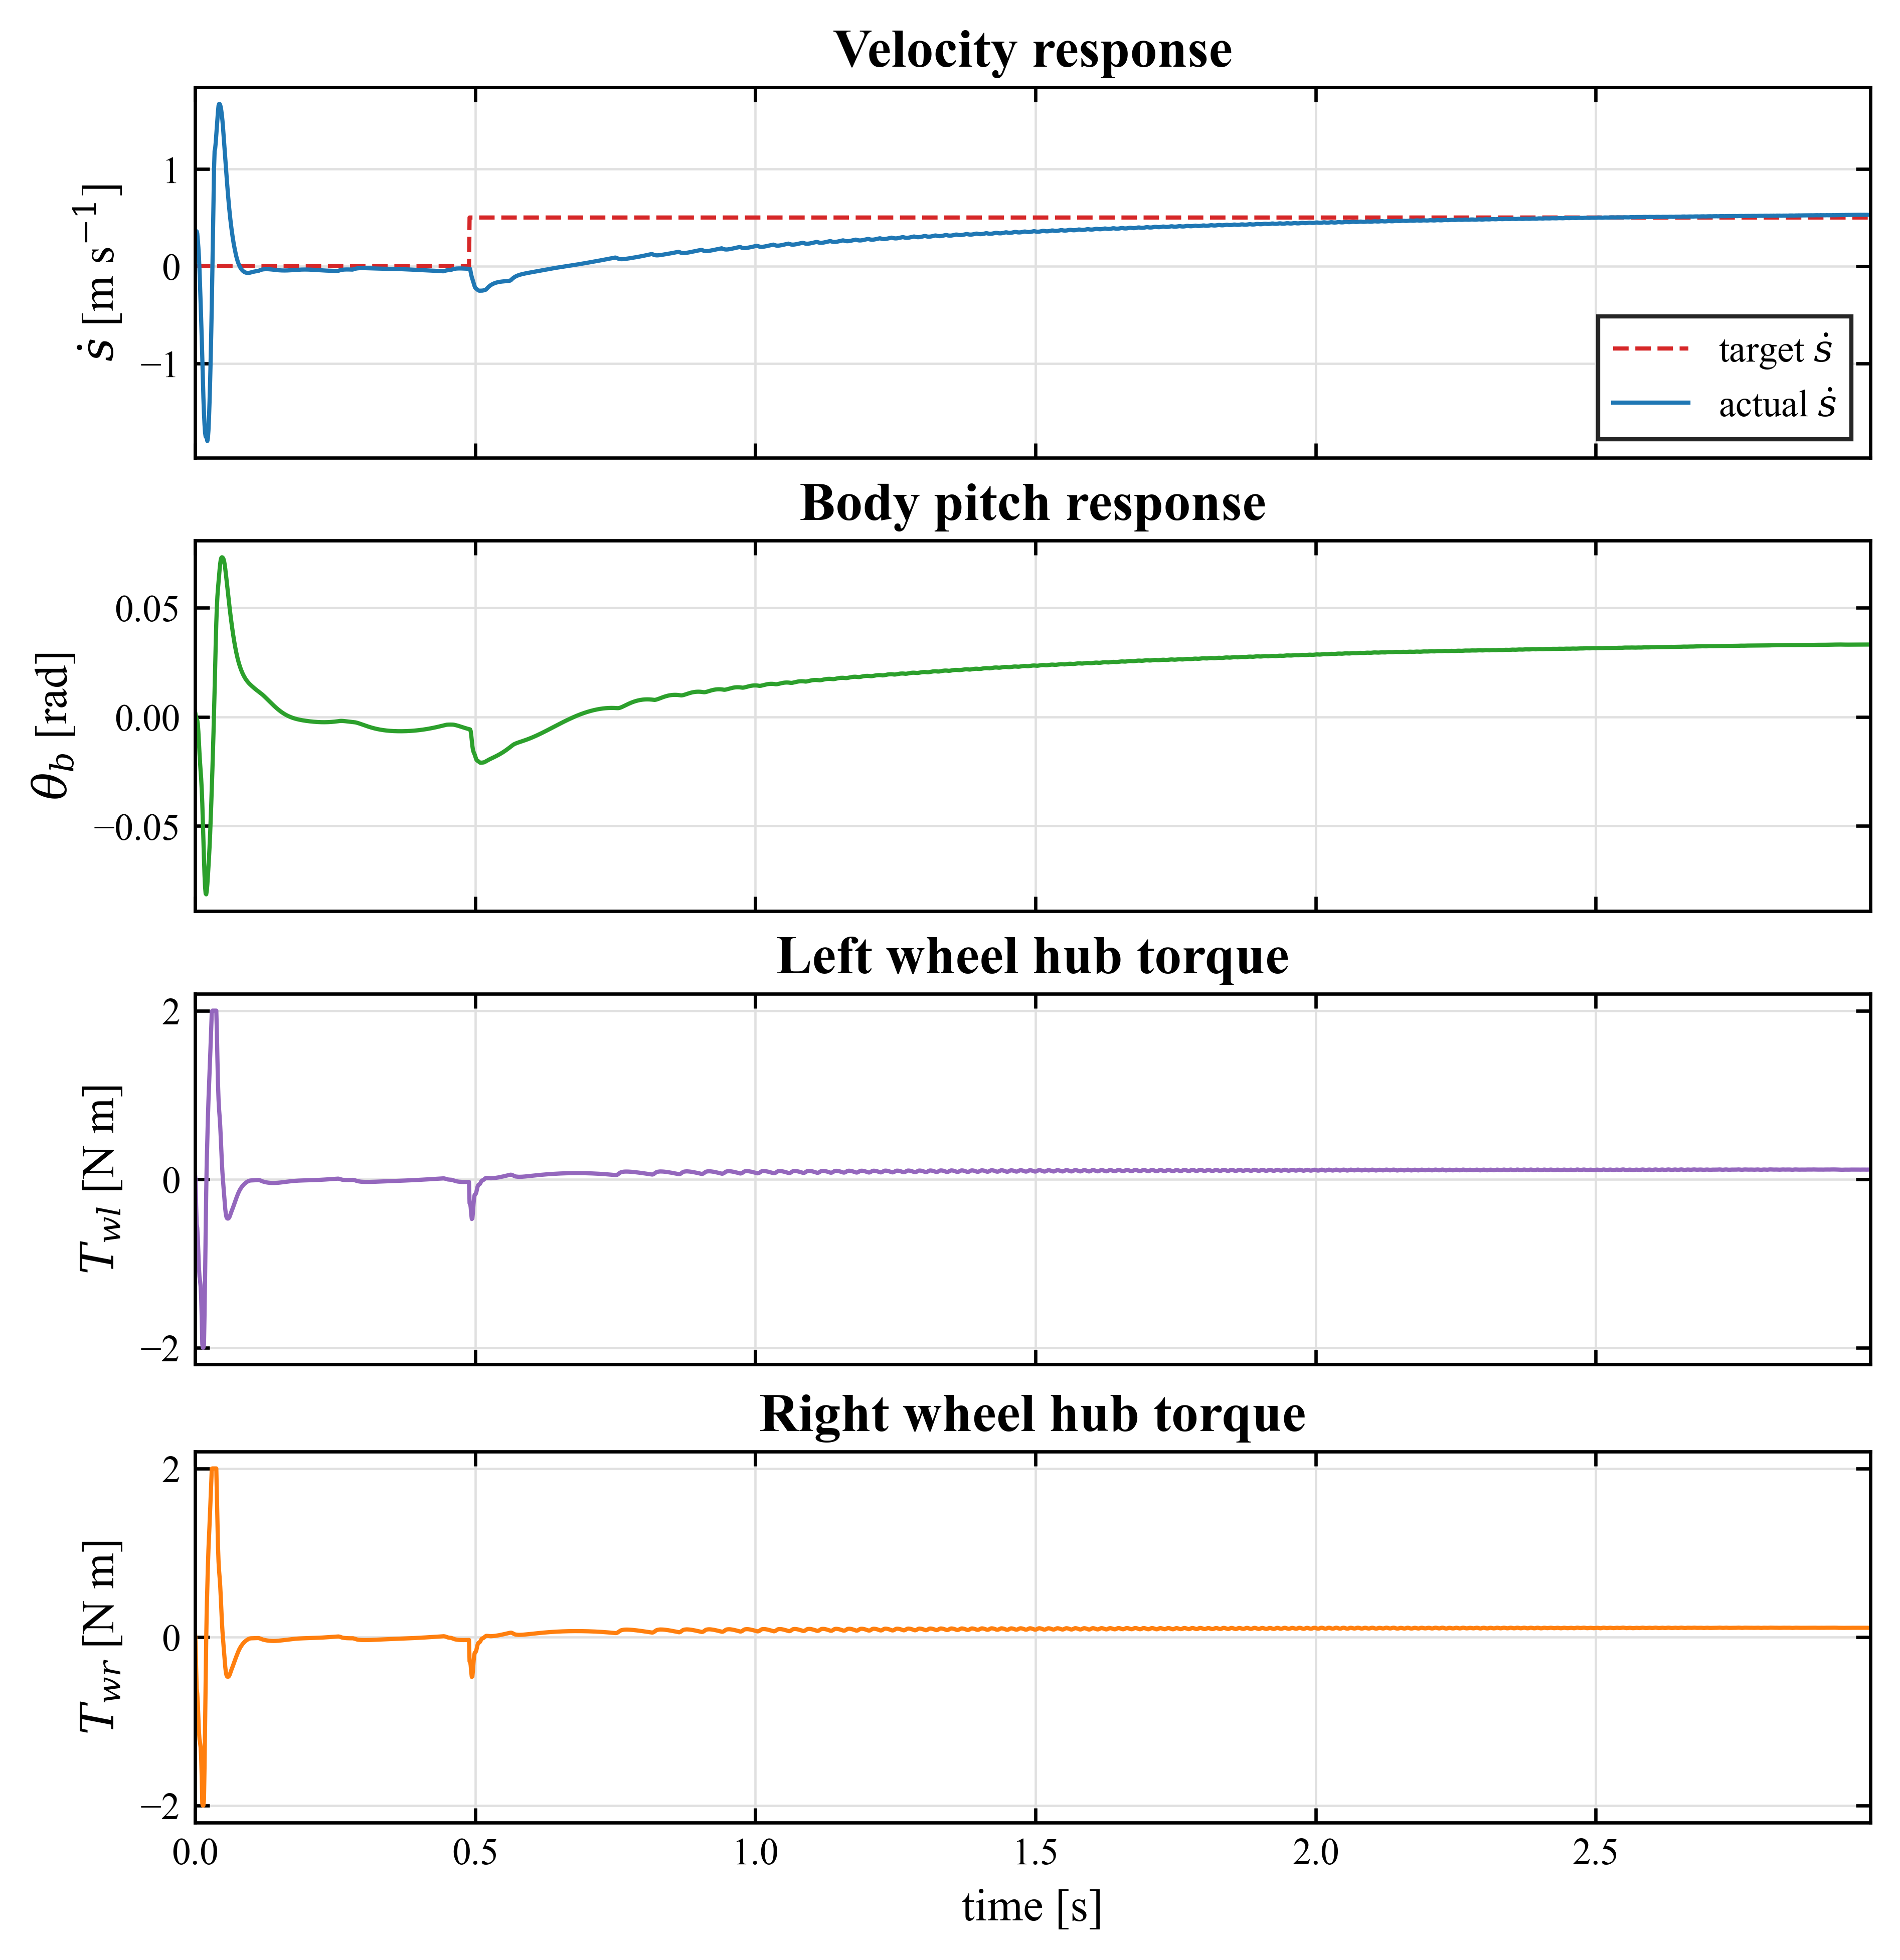
\includegraphics[width=1.0\textwidth]{figures/ch04/velocity_tracking.png}
  \caption{速度跟踪工况下的闭环响应。从上至下分别为前进速度、机体俯仰角、轮端力矩}
  \label{fig:velocity-tracking}
\end{figure}

仿真结果显示实际速度对参考速度的跟随误差在2s后逐渐收敛为0，速度切换时的俯仰角峰值为$0.05rad$， 轮端力矩峰值在$2N\cdot m$内。
说明所设计的 LQR 权重能够在速度跟踪和姿态稳定之间取得可接受的折中。
并且由于轮式倒立摆建模的非最小相位特性，机体想要获得向前的加速度必须先将机身后仰将重心调整至轮轴前方，随后再通过轮端力矩产生加速效果。
由图 \ref{fig:velocity-tracking}可看出$\dot{s}$先为负值后迅速收敛至$0.5m/s$附近，能够反映 LQR 对非最小相位特性的处理能力。

\subsection{扰动恢复}

扰动恢复仿真用于评估控制器对外部冲击的鲁棒性。仿真中保持机器人处于原地平衡状态，分别对机体施加竖直方向和水平方向$2N$的短时脉冲扰动。竖直扰动主要考察 VMC 腿长支撑通道对瞬时载荷变化的缓冲能力，水平扰动主要考察 LQR 平衡控制器对机体俯仰偏差和前后运动趋势的恢复能力。扰动施加位置与方向如\figref{fig:vertical-impulse-scene} 和\figref{fig:horizon-impulse-scene} 所示。

\begin{figure}[H]
  \centering
  \begin{subfigure}[t]{0.38\textwidth}
    \centering
    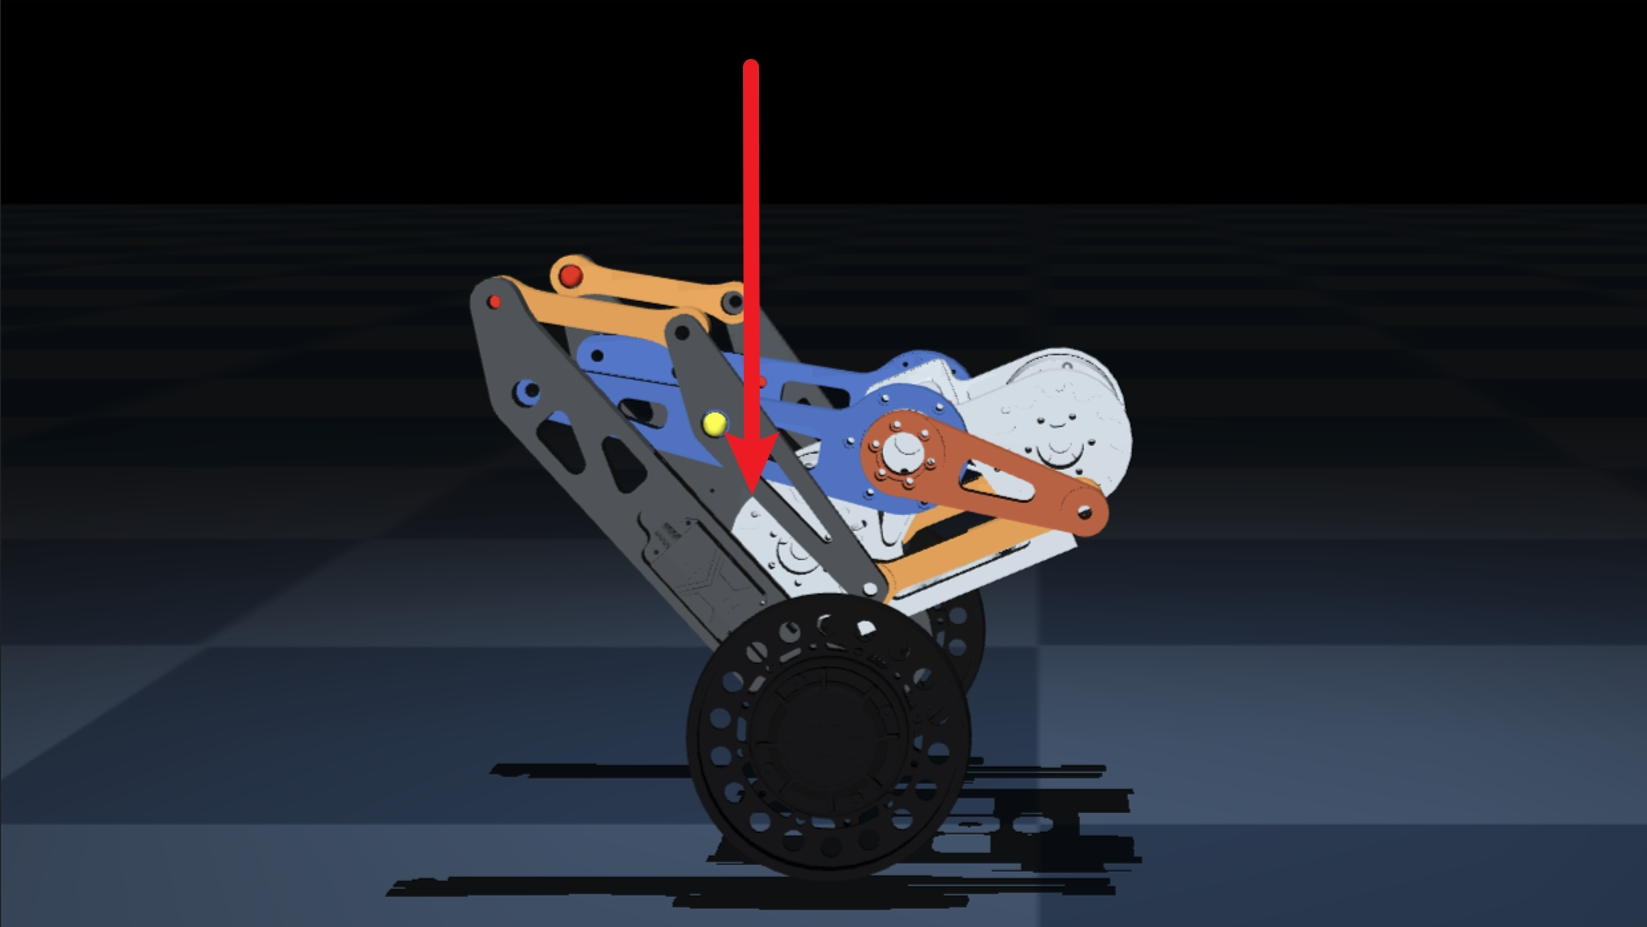
\includegraphics[width=\textwidth]{figures/ch04/vertical_impulse.jpg}
    \caption{竖直脉冲扰动}
    \label{fig:vertical-impulse-scene}
  \end{subfigure}
  \hspace{0.08\textwidth}
  \begin{subfigure}[t]{0.38\textwidth}
    \centering
    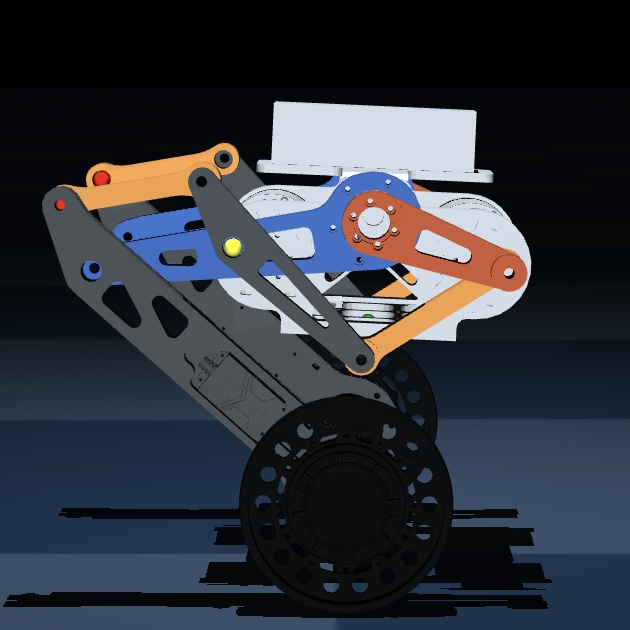
\includegraphics[width=\textwidth]{figures/ch04/horizon_impulse.jpg}
    \caption{水平脉冲扰动}
    \label{fig:horizon-impulse-scene}
  \end{subfigure}
  \caption{不同方向脉冲扰动仿真场景}
  \label{fig:impulse-scene}
\end{figure}

\begin{figure}[H]
  \centering
  \begin{subfigure}[t]{0.49\textwidth}
    \centering
    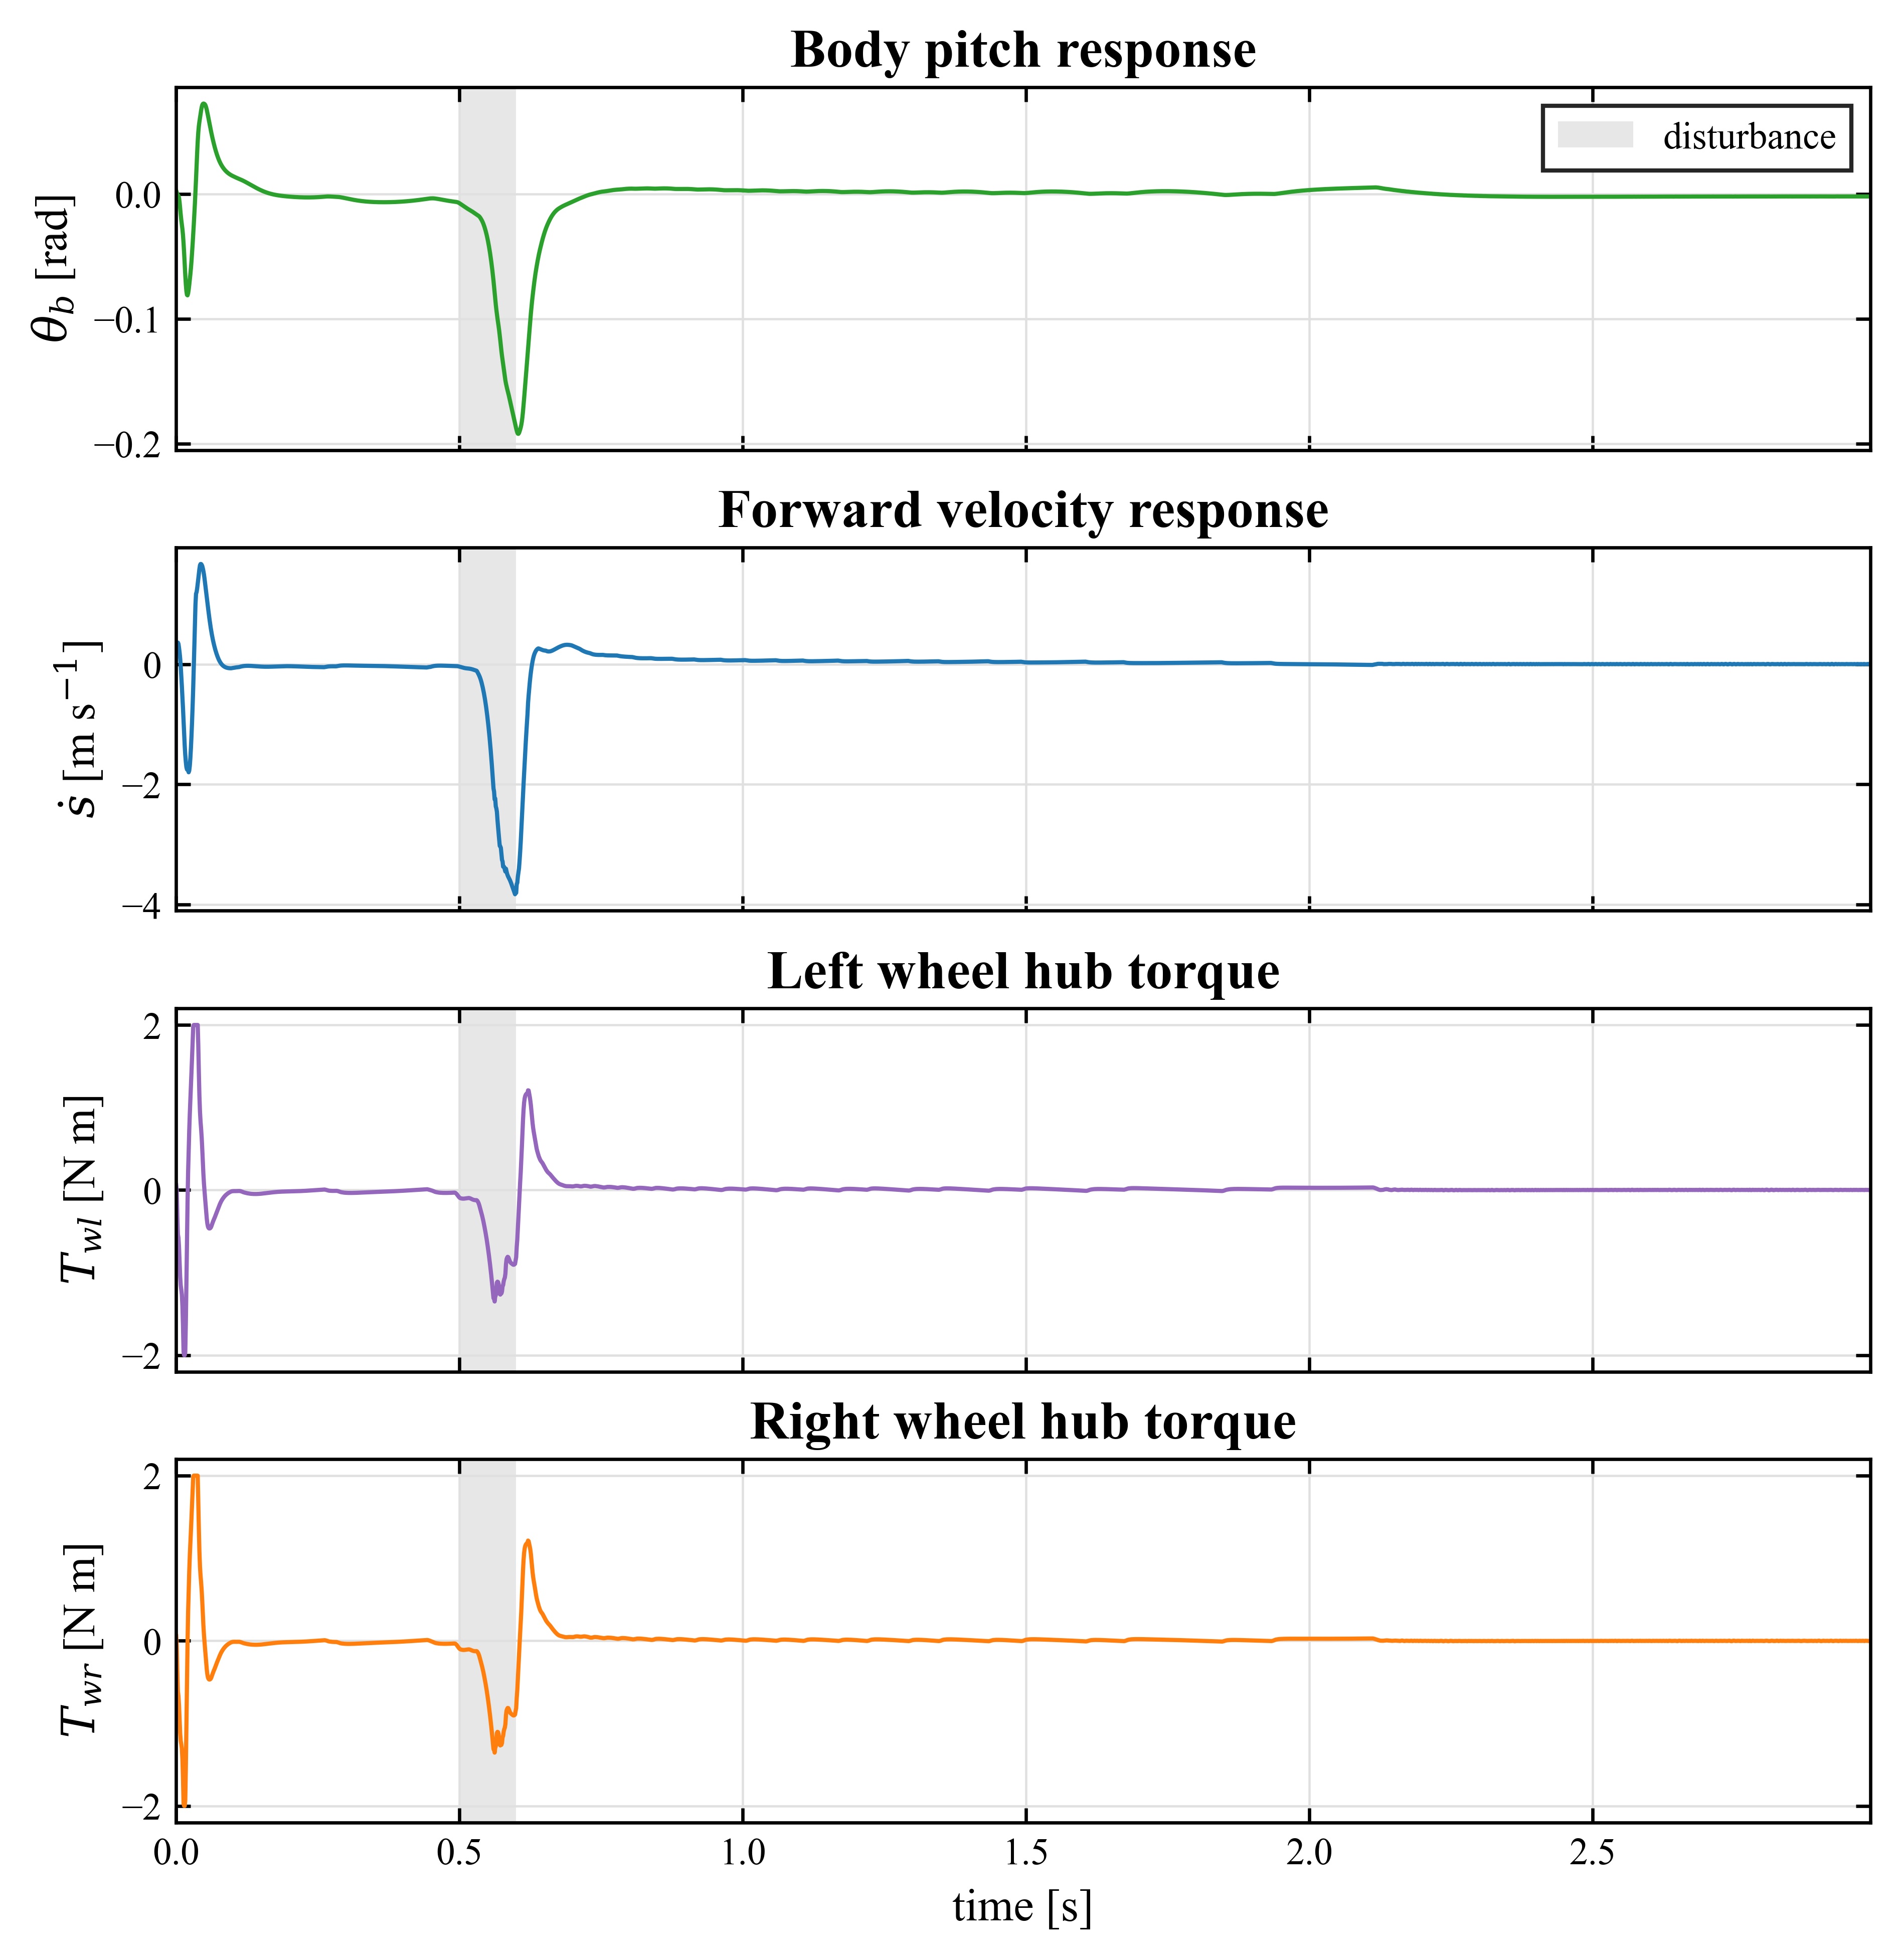
\includegraphics[width=\textwidth]{figures/ch04/vertical_impulse_out.png}
    \caption{竖直脉冲扰动响应}
    \label{fig:vertical-impulse-out}
  \end{subfigure}
  \hfill
  \begin{subfigure}[t]{0.49\textwidth}
    \centering
    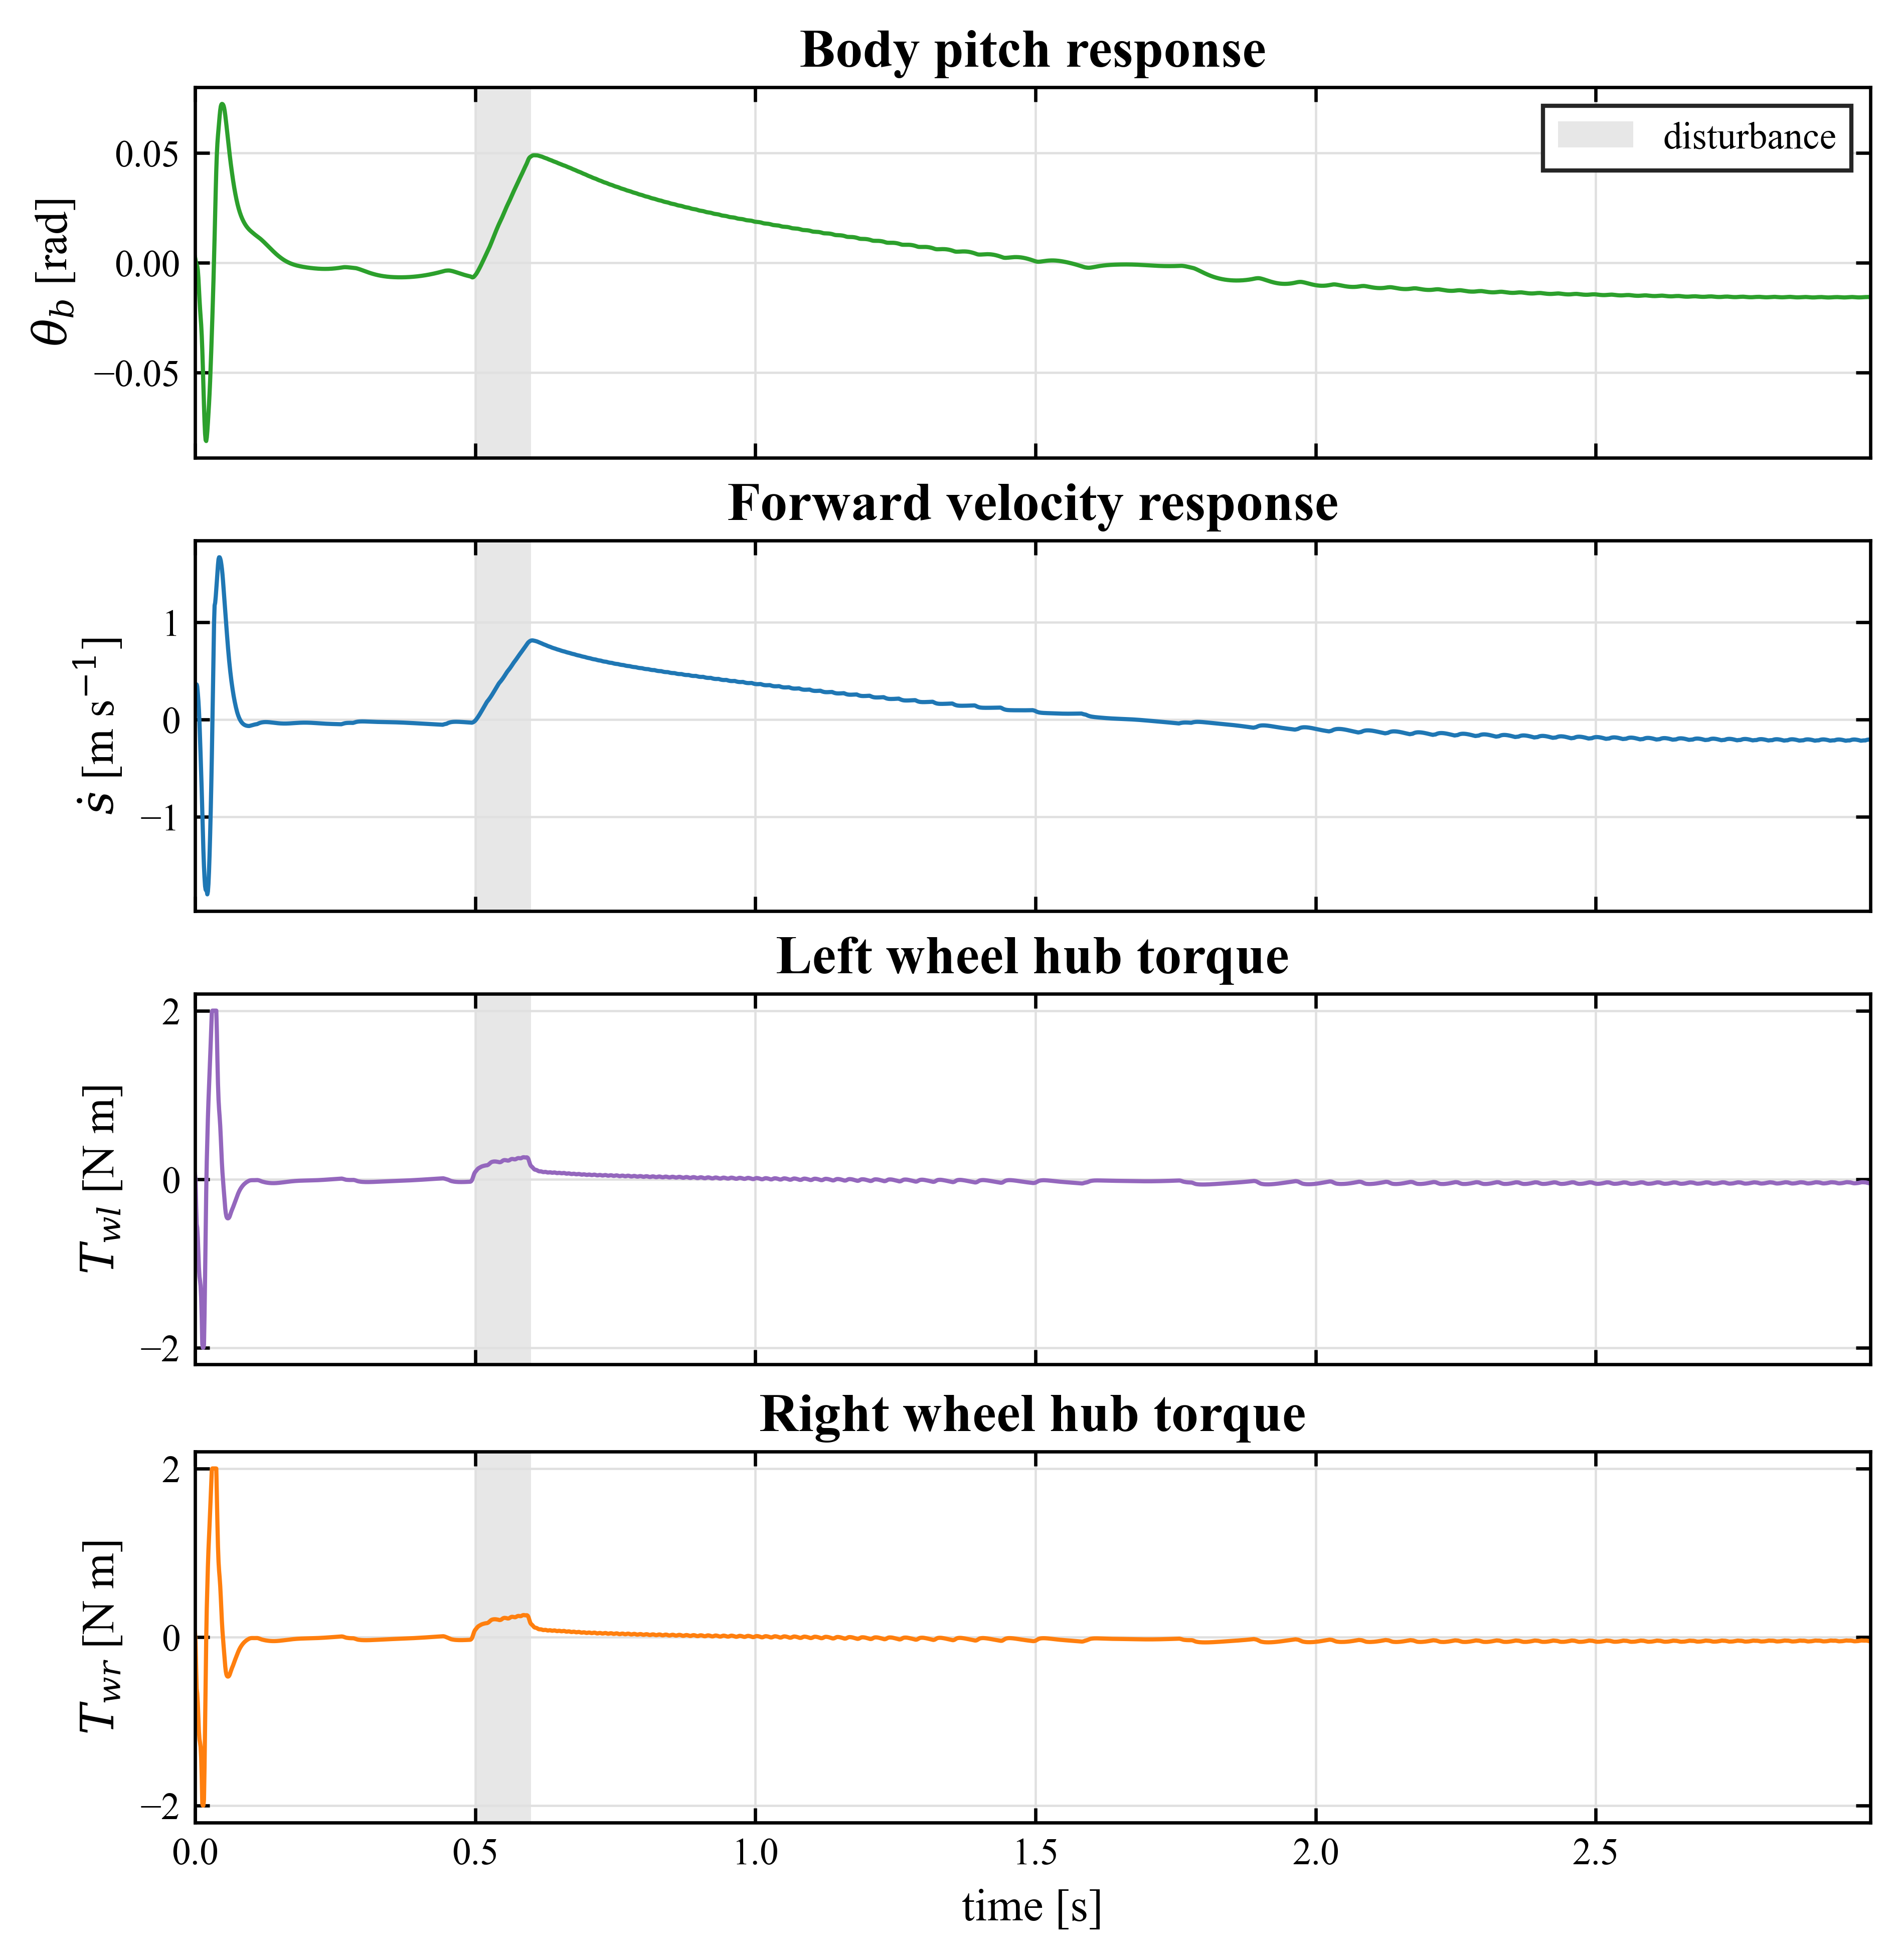
\includegraphics[width=\textwidth]{figures/ch04/horizon_impulse_out.png}
    \caption{水平脉冲扰动响应}
    \label{fig:horizon-impulse-out}
  \end{subfigure}
  \caption{不同方向脉冲扰动下的闭环响应}
  \label{fig:impulse-disturbance-out}
\end{figure}

由\figref{fig:vertical-impulse-out} 可见，竖直扰动施加后，腿部轴向力首先出现短时峰值，随后在阻尼项作用下逐渐回到稳定支撑范围，左右腿长也未产生持续发散。该结果说明 VMC 腿长通道能够对瞬时竖直载荷进行缓冲。由\figref{fig:horizon-impulse-out} 可见，水平扰动施加后，机体俯仰角和前进速度出现瞬时偏差，轮端力矩随即产生反向调节，使机器人重新回到平衡状态。两类扰动结果表明，本文控制器在不同方向外部冲击下均具有一定恢复能力。

\subsection{腿长控制验证}

腿长控制验证用于检查 VMC 腿长通道对不同期望腿长的响应能力。仿真中保持机器人处于原地平衡状态，前进速度参考取 $\dot{s}_d=0$，分别对左右腿公共期望腿长 $l_d$ 施加阶跃激励和正弦激励。阶跃激励用于观察腿长指令突变时的快速调节能力，正弦激励用于观察连续高度变化下的跟踪能力。两类工况能够直接反映式\eqref{eq:leg-force-law} 所构造的虚拟弹簧阻尼控制律是否能够驱动腿部机构完成高度调节，并检验腿长变化过程中机体俯仰角和腿部轴向力是否保持在合理范围内。

\begin{figure}[H]
  \centering
  \begin{subfigure}[t]{0.49\textwidth}
    \centering
    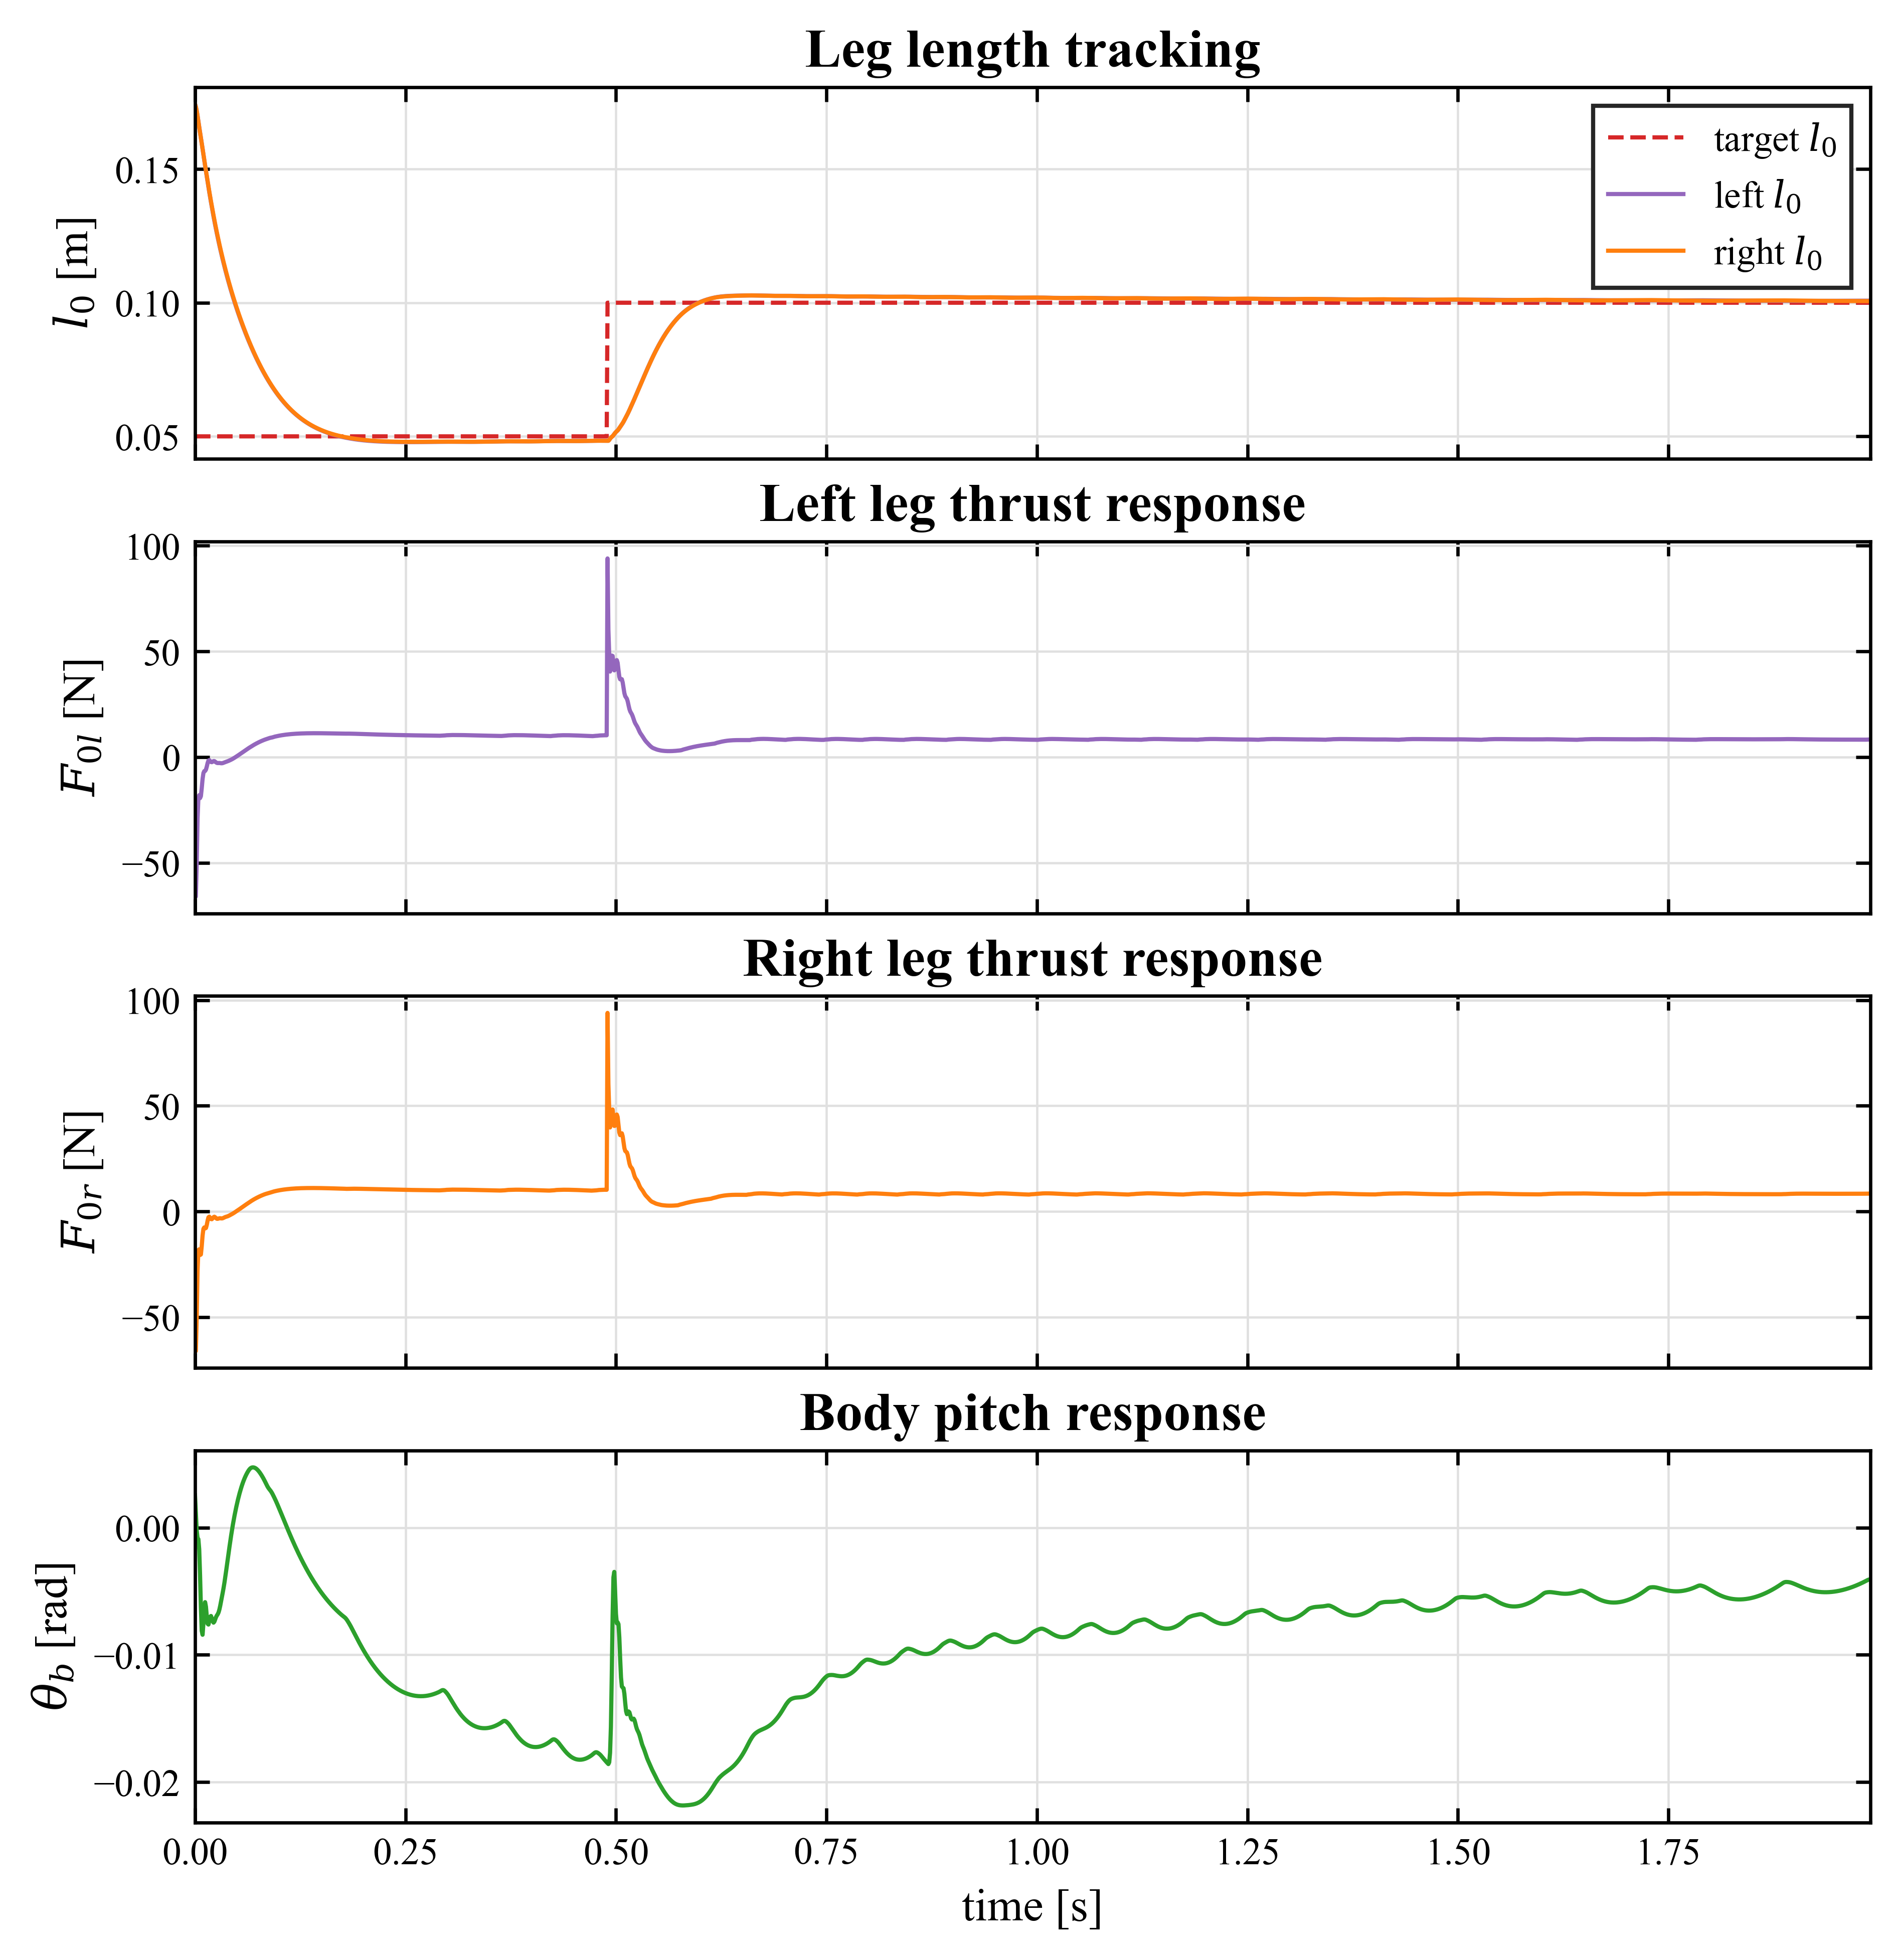
\includegraphics[width=\textwidth]{figures/ch04/step_velocity.png}
    \caption{阶跃腿长指令响应}
    \label{fig:leg-length-step}
  \end{subfigure}
  \hfill
  \begin{subfigure}[t]{0.49\textwidth}
    \centering
    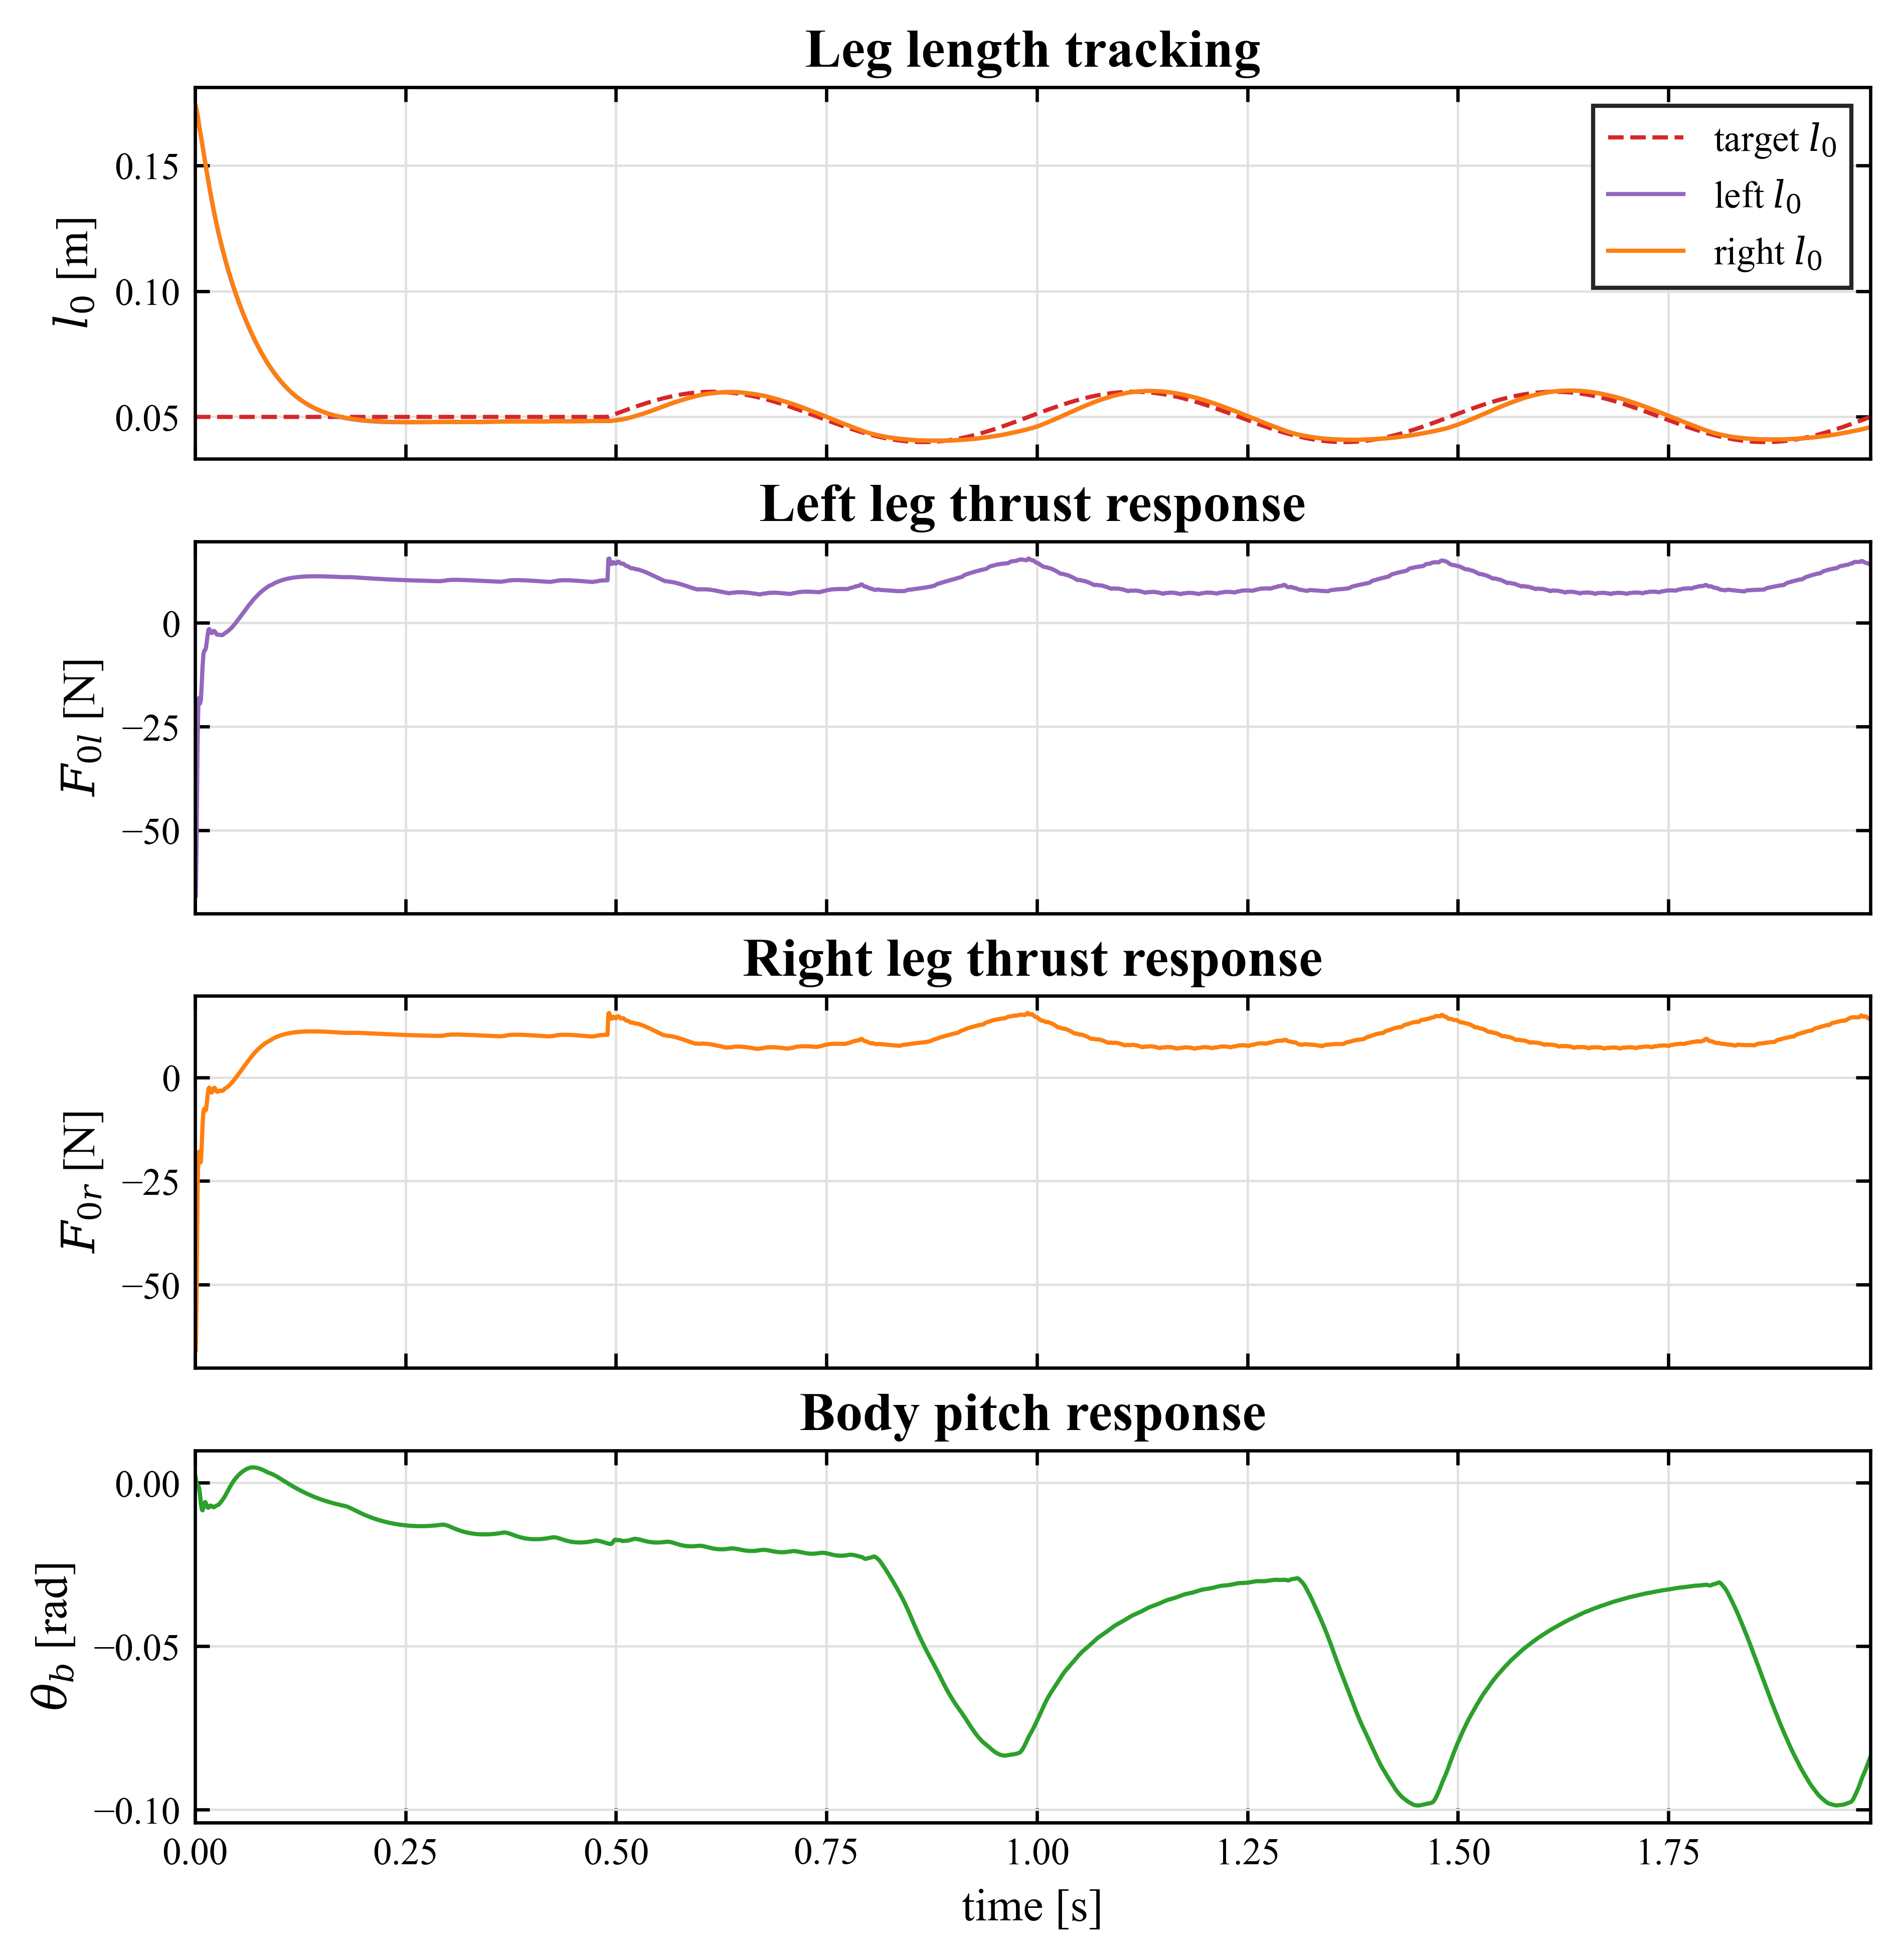
\includegraphics[width=\textwidth]{figures/ch04/sine_velocity.png}
    \caption{正弦腿长指令响应}
    \label{fig:leg-length-sine}
  \end{subfigure}
  \caption{不同腿长激励下的 VMC 腿长控制响应。从上至下分别为腿长跟踪、左腿轴向力、右腿轴向力和机体俯仰角}
  \label{fig:leg-length-excitation}
\end{figure}

由\figref{fig:leg-length-step} 可见，当期望腿长在 $0.5\,\mathrm{s}$ 附近由低位腿长切换至较高腿长时，左右腿实际腿长能够快速跟随参考值并在短时间内收敛。腿长突变瞬间，左右腿轴向力出现短时峰值，这是虚拟弹簧阻尼器为克服腿部惯性和支撑载荷而产生的瞬态输出；随后轴向力回到稳定支撑范围。机体俯仰角仅出现小幅波动，说明腿长阶跃调节未破坏整机平衡。

由\figref{fig:leg-length-sine} 可见，在正弦期望腿长输入下，左右腿实际腿长能够连续跟随目标曲线，虽然存在一定相位滞后，但整体变化趋势与参考信号一致。左右腿轴向力随期望腿长变化呈周期性调节，反映 VMC 控制器能够根据腿长误差持续修正支撑力。该结果说明本文腿长控制器不仅能够响应离散高度切换，也能够支持连续高度调节，为后续越障、缓冲和姿态调节动作提供了基础。

\section{本章小结}

本章围绕双轮足机器人控制系统的实际需求，提出了一种面向嵌入式实时实现的 LQR-VMC 平衡控制算法。
首先，从控制目标和工程约束出发，说明了采用“LQR 运动 + VMC 腿长支撑 + 滚转补偿”这一分层架构的原因；随后，基于第三章的建模结果构建了运动控制器所需的线性状态空间模型，并设计了 LQR 反馈律；在此基础上，通过 VMC 完成腿长支撑控制，并将 LQR 输出的腿摆控制量一并映射到关节空间，同时利用滚转辅助控制实现左右腿长参考修正；最后，给出了控制系统的状态估计与在线工作流程，并说明了 MuJoCo 仿真验证的模型构建、工况设置和数据记录方法。上述内容共同构成了本文后续物理样机实验所依赖的控制系统实现基础。
